\chapter[Tracking Rodinia into the Neoproterozoic: new paleomagnetic constraints from the Jacobsville Formation][Tracking Rodinia into the Neoproterozoic]{Tracking Rodinia into the Neoproterozoic: new paleomagnetic constraints from the Jacobsville Formation}

\let\thefootnote\relax\footnote{This chapter is published as a peer-reviewed manuscript: Zhang, Y., Hodgin, E.B., Mohr, M.T., Alemu, T.B., Pierce, J., Fuentes, A.J., Swanson-Hysell, N.L. (2024). Tracking Rodinia into the Neoproterozoic: new paleomagnetic constraints from the Jacobsville Formation. Tectonics. doi: \url{https://doi.org/10.1029/2023TC007866.}}

\section{Abstract}
The paleogeography of Laurentia throughout the Neoproterozoic is critical for reconstructing global paleogeography due to its central position in the supercontinent Rodinia. We develop a new paleomagnetic pole from red siltstones and fine-grained sandstones of the early Neoproterozoic Jacobsville Formation which is now constrained to be ca. 990 Ma in age. High-resolution thermal demagnetization experiments resolve detrital remanent magnetizations held by hematite. These directions were reoriented within siltstone intraclasts and pass intraformational conglomerate tests---giving confidence that the magnetization is detrital and primary. An inclination-corrected mean paleomagnetic pole position for the Jacobsville Formation indicates that Laurentia's motion slowed down significantly following the onset of the Grenvillian orogeny. Prior rapid plate motion associated with closure of the Unimos Ocean between 1110 and 1090 Ma transitioned to slow drift of Laurentia across the equator in the late Mesoproterozoic to early Neoproterozoic. We interpret the distinct position of this well-dated pole from those in the Grenville orogen that have been assigned a similar age to indicate that the ages of the poles associated with the Grenville Loop likely need to be revised to be younger due to prolonged exhumation. 

\section{Introduction}

The extensively studied paleomagnetic records of ca. 1109 to 1084 Ma volcanics and intrusions associated with the North American Midcontinent Rift provide crucial constraints on the paleogeography of Laurentia in the late Mesoproterozoic Era \citep{Halls1982a, Fairchild2017a, Swanson-Hysell2019a}. The resulting sequence of poles known as the Keweenawan Track is a central record for reconstructing the assembly of the ancient supercontinent Rodinia \citep{Evans2021b}. An advantage of intracratonic magmatic events, such as those preserved in the Midcontinent Rift, is that they lead to emplacement of igneous rocks that can readily retain primary thermal remanent magnetization (TRM) that can be confidently associated with the emplacement age of the unit. However, following the development of the Midcontinent Rift, there was a $\sim$300 Myr quiescence in known intracratonic magmatic activity in Laurentia that lasted until the emplacement of the ca. 775 Ma Gunbarrel large igneous province \citep{Harlan2003a, Mackinder2019a, Swanson-Hysell2021c}. The lack of Laurentian rocks with primary TRM in the early Neoproterozoic has led paleogeographic reconstructions to be reliant on magnetizations acquired by rocks that were metamorphosed during the ca. 1090 to 980 Ma Grenvillian orogeny \citep{Rivers2008a, Rivers2012a, Swanson-Hysell2023a}. However, rocks within the orogen acquired their magnetizations during exhumation after peak metamorphic conditions \citep{McWilliams1975a}. As a result, the timing of remanence acquisition needs to be constrained through the more difficult task of dating cooling associated with exhumation. This gap in well-dated paleomagnetic poles for Laurentia in the late Mesoproterozoic to mid-Neoproterozoic contributes to uncertainty in paleogeography at that time including the configuration of the supercontinent Rodinia.

\begin{figure*}[h!]
\centering
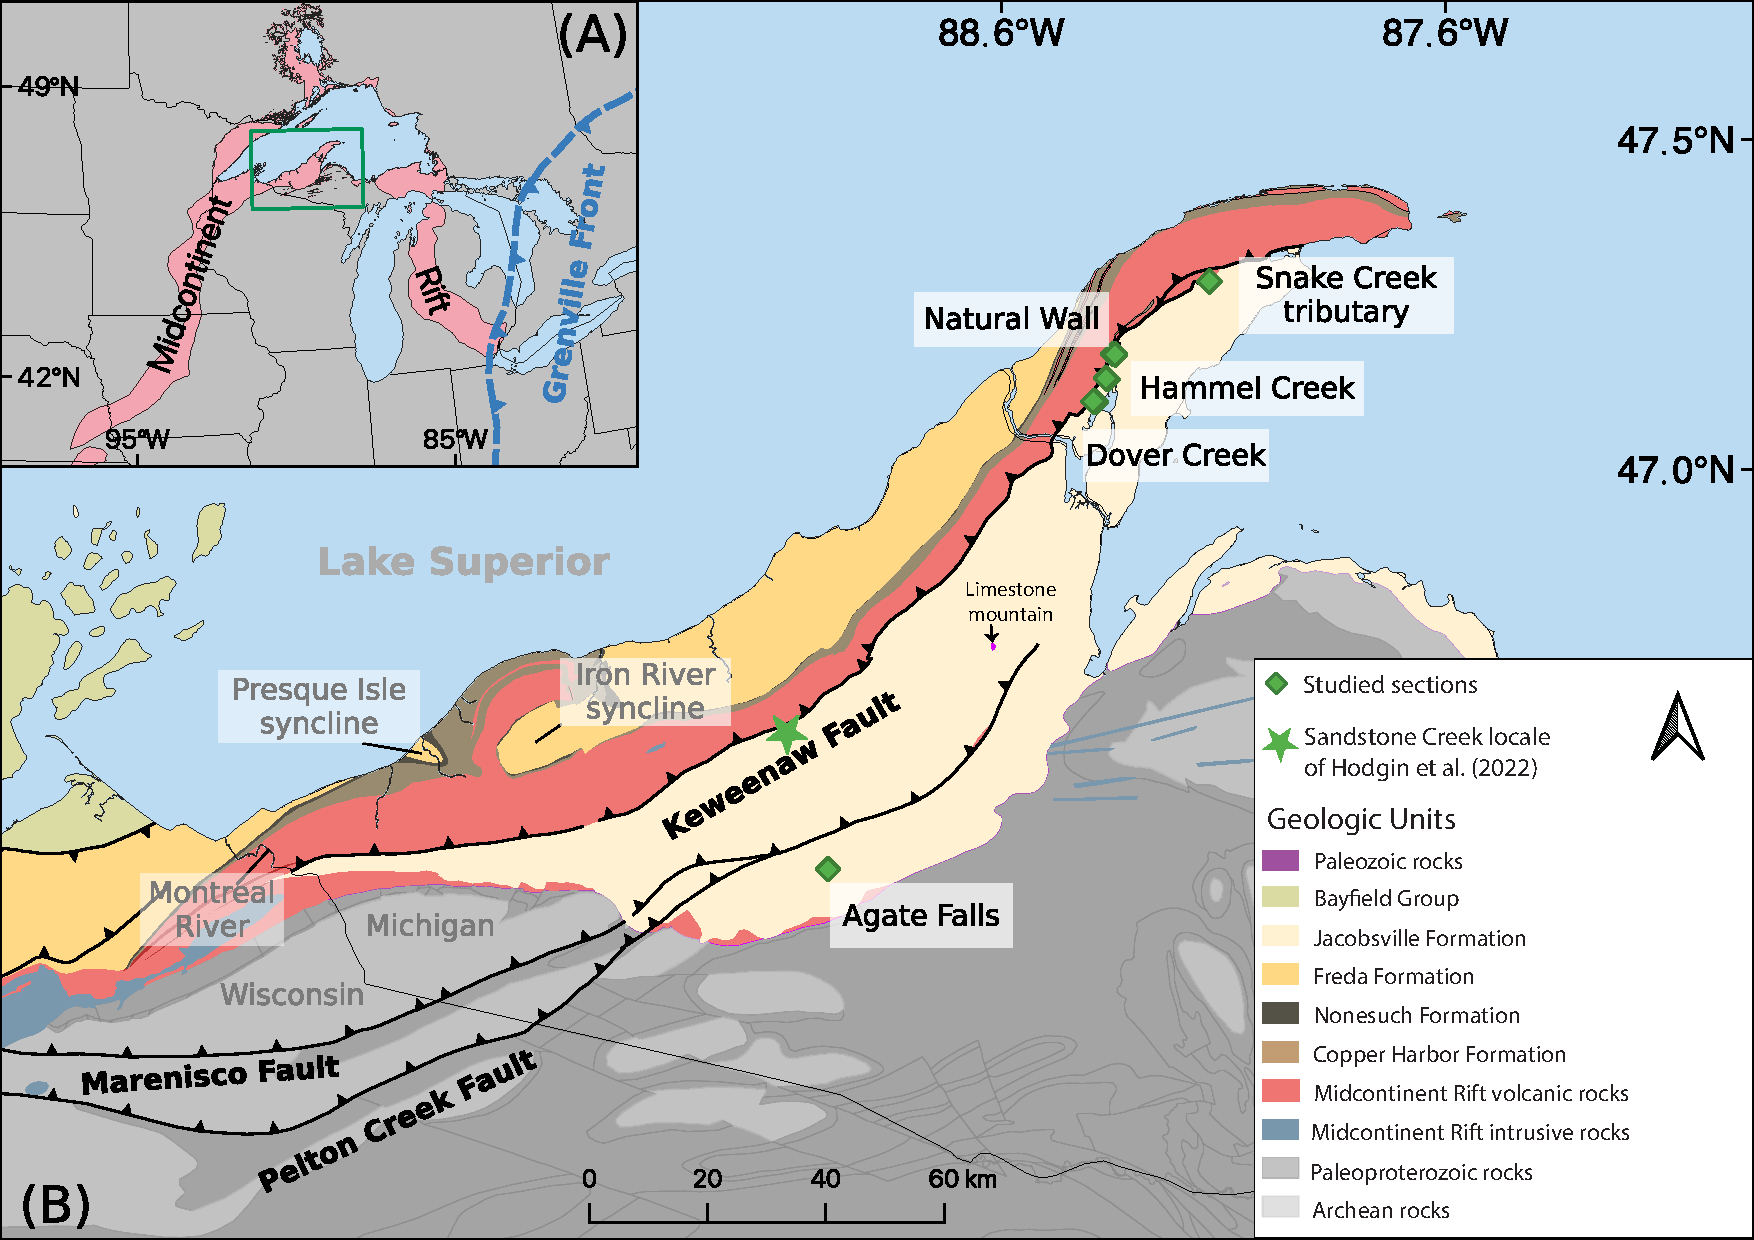
\includegraphics[width=\textwidth]{figure/Zhang2024a/Geologic_map.pdf}
\caption[Overview map of the Midcontinent Rift and the geologic map of the Jacobsville Formation and associated units]{(A) Regional map showing the extent of the Midcontinent Rift and the location of the Grenville Front relative to the study area. The inset green box shows the extent of panel B. (B) Geologic map of northern Michigan and Wisconsin showing Midcontinent Rift igneous and sedimentary rocks, sedimentary rocks of the Jacobsville Formation and Bayfield Group, other older Paleoproterozoic and Archean rocks, and major post-rift thrust faults. The location of the Jacobsville stratigraphic sections in this study are shown with green diamonds. Map modified from \cite{Nicholson2004a}.}
\label{fig:Chap_Jacobsville_Geologic_map}
\end{figure*}

Paleomagnetic poles can also be developed from sedimentary rocks deposited in basins. Sedimentary rocks of the Oronto Group deposited during post-rift thermal subsidence following the bulk of Midcontinent Rift magmatic activity provide paleomagnetic poles that extend the Keweenawan Track to ca. 1070 Ma \citep{Henry1977a, Slotznick2023a}. While there are some contemporaneous basins in northern Laurentia \citep{Greenman2021a}, there is minimal basin development within Laurentia following the Grenvillian orogeny until the Rodinia supercontinent began to rift apart ca. 770 Ma \citep{Macdonald2023a}. 

One rare preservation of an early Neoproterozoic sedimentary succession in Laurentia's interior is the Jacobsville Formation (Fig. \ref{fig:Chap_Jacobsville_Geologic_map}; \citealp{Hamblin1958a, Hodgin2022a, DeGraff2022a}). U-Pb detrital zircon dates developed through chemical abrasion–isotope dilution–thermal ionization mass spectrometry (CA-ID-TIMS) of 1003.21 $\pm$ 2.23 Ma and 992.51 $\pm$ 0.64 Ma (2$\sigma$ analytical uncertainty) constrain the maximum deposition age of the Jacobsville Formation \citep{Hodgin2022a}. A 985.5 $\pm$ 35.8 Ma (2$\sigma$ analytical uncertainty) U-Pb date from calcite veins within the Keweenaw fault provides a minimum age constraint on Jacobsville deposition, as the Jacobsville Formation is folded in the footwall against Midcontinent rift volcanics in the hanging wall. Together, these dates bracket the depositional age of the Jacobsville Formation and constrain it to be ca. 990 Ma \citep{Hodgin2022a}. These results support the interpretation that the formation was deposited within a syn-orogenic basin during the Rigolet phase of the Grenvillian orogen and was then deformed during the same orogenic phase.

The Jacobsville Formation contains abundant hematite-bearing sandstone and siltstone which have the potential to record a key pole in Laurentia's apparent polar wander path (APWP) \citep{Dubois1962a, Roy1978a}. \cite{Roy1978a} conducted a paleomagnetic study that developed a pole which has been used in paleogeographic syntheses where it has been assigned variable ages including an age of ca. 1020 Ma based on APWP extrapolation \cite[e.g.][]{Li2008a}. However, the uncertainty in the age of the magnetization combined with a lack of field tests, and no application of inclination correction have resulted in the pole not being included in recent curated compilations \cite[e.g.][]{Evans2021a}. Obtaining high-quality paleomagnetic data, including robust field tests, motivates the development of new data from the Jacobsville Formation. 

In this study, we investigate five stratigraphic sections of the Jacobsville Formation on and near the Keweenaw Peninsula, Michigan, USA (Figs. \ref{fig:Chap_Jacobsville_Geologic_map} and \ref{fig:strat_column}). These sections were chosen given the abundance of fine-grained siliciclastic lithologies where magnetization can be constrained through intraclast conglomerate field tests. Additionally, they are within the continuous bedrock belt from which chronostratigraphic constraints have been developed. In contrast to fluvial sandstones in other exposures such as in the eastern Lake Superior region near Sault Ste. Marie, the maximum and minimum depositional ages of these sections can be more confidently constrained. 

Within sampled lithologies, high-resolution thermal demagnetization isolates primary detrital remanent magnetization (DRM) from secondary chemical remanent magnetization (CRM). This interpretation is supported by the DRM directions passing intraformational conglomerate tests on siltstone intraclasts that were ripped-up and remobilized within the fluvial depositional environment. A paleomagnetic fold test further constrains the timing of DRM acquisition to predate the folding of the Jacobsville Formation in the footwall of the Keweenaw fault soon after deposition. With these data, we develop a new inclination-corrected paleomagnetic pole for the Jacobsville Formation based on a large number of samples that gives new constraints on the paleogeographic position of Laurentia in the earliest Neoproterozoic.

\section{Geologic setting}

The ca. 1109 Ma to 1084 Ma North American Midcontinent Rift is a major intracontinental rift system that extends over 2000 km through the Laurentia craton (Fig. \ref{fig:Chap_Jacobsville_Geologic_map}). Following the end of active extension in the rift, thermal subsidence resulted in the accumulation of $>$4 km of ca. 1085-1050 Ma Oronto Group strata that are both intercalated with the youngest volcanics and deposited atop them (Fig. \ref{fig:Chap_Jacobsville_Geologic_map}; \citealp{Daniels1982a, Cannon1989a}). Subsequently, the rift was inverted as contraction associated with the ca. 1090-980 Ma Grenvillian Orogeny on the eastern margin of Laurentia (Fig. \ref{fig:Chap_Jacobsville_Geologic_map}) propagated into Laurentia's interior \citep{Cannon1993a, Cannon1994a, Hodgin2022a, Swanson-Hysell2023a}. 

During rift inversion, Midcontinent Rift volcanic and sedimentary rocks were uplifted along with Paleoproterozoic and Archean lithologies via thrust faults such as the Marenisco fault, forming the crustal-scale Montreal River monocline (Fig. \ref{fig:Chap_Jacobsville_Geologic_map}; \citealp{Cannon1993a}). Rb-Sr biotite thermochronology data of \cite{Cannon1993a} show Archean lithologies within the Montreal River monocline to have been exhumed to mid to shallow crustal temperatures ($\sim$270\textdegree C) by ca. 1050 Ma. The Jacobsville Formation overlies an angular unconformity that developed on lithologies that were exhumed through this earlier episode of contractional deformation associated with Grenvillian orogenesis (Fig. \ref{fig:Chap_Jacobsville_Geologic_map}; \citealp{Hamblin1958a, Cannon1993a, Kalliokoski1982a}). Conglomeratic facies occur in the basal Jacobsville Formation, with clasts derived from locally uplifted basement lithologies \citep{Irving1885a, Hamblin1958a, Kalliokoski1982a}.

Bedding planes in the Jacobsville Formation typically have shallow dips. The exception to these near-horizontal orientations is proximal to reverse faults such as the Keweenaw fault (Fig. \ref{fig:Chap_Jacobsville_Geologic_map}) where the Jacobsville Formation was occasionally deformed into monoclinal drag folds resulting in steeply tilted to overturned beds (Fig. \ref{fig:Chap_Jacobsville_Geologic_map}; \citealp{Irving1885a, Cannon2001a}). Recent mapping of the Jacobsville Formation also found that it sometimes onlaps the Midcontinent Rift volcanics within or adjacent to en echelon fault branches of the Keweenaw fault system near the northern end of the Keweenaw Peninsula \citep{Tyrrell2019a, Mueller2021a}. These observations are consistent with the interpretation that there was deposition of Jacobsville Formation sediments during faulting.

\subsection{Overview of Jacobsville sedimentology and stratigraphy}

The Jacobsville Formation is a fluvial succession of feldspathic and quartzose conglomerates, sandstones, siltstones, and shales devoid of lava flows or cross-cutting igneous dikes although internal clastic dikes are present \citep{Hamblin1958a}. Sandstones of the Jacobsville Formation are more quartz-rich with generally fewer lithic fragments than sandstones of the Oronto Group such that they can typically be classified as subarkose to quartz arenites (Fig. \ref{fig:Field_photo}; \citealp{Hamblin1958a, Ojakangas2002a}). While much of the Jacobsville Formation is dominated by sandstone channel deposits, there are clay-rich siltstones that formed in overbank settings that are a major focus of this study.

\begin{figure*}[h!]
\centering
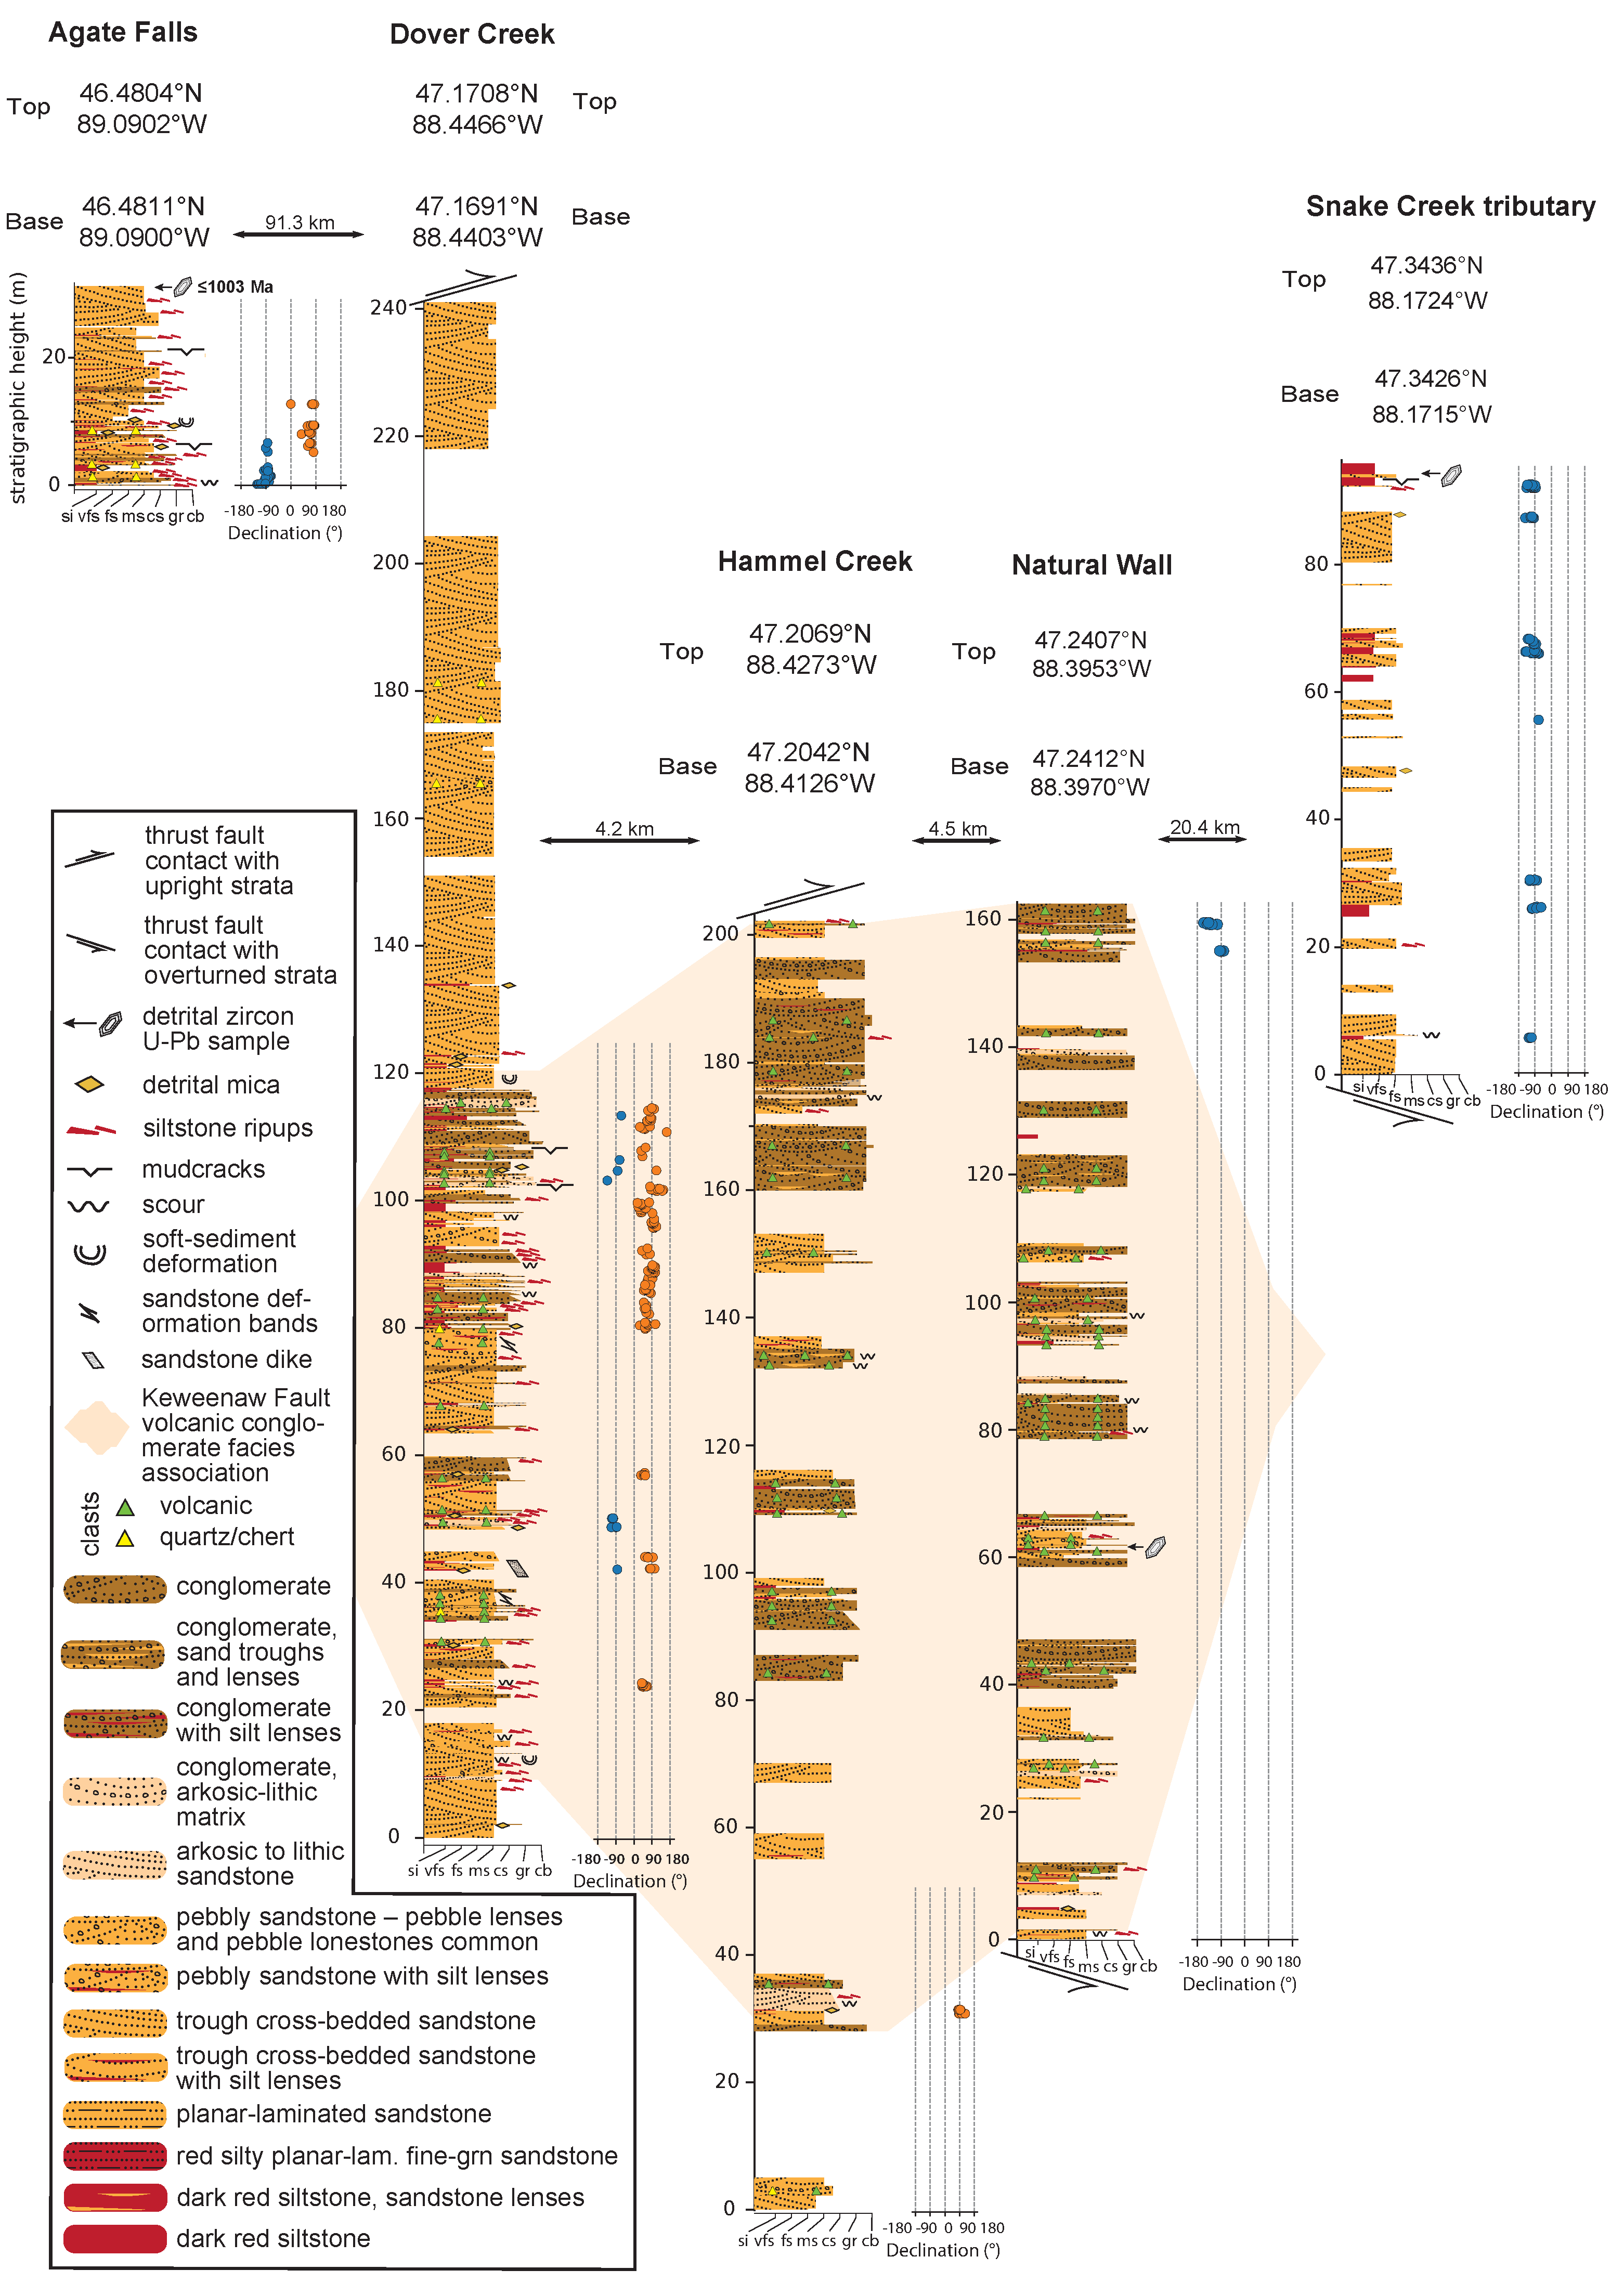
\includegraphics[width=0.6\textwidth]{figure/Zhang2024a/Jacobsville_Sections_v6.pdf}
\caption[Lithostratigraphy and magnetostratigraphy for studied sections of the Jacobsville Formation]{\footnotesize Lithostratigraphy and magnetostratigraphy for studied sections of the Jacobsville Formation in northern Michigan, USA. GPS locations for the base and top of the sections are noted. Paleomagnetic sampling focused on the dark red siltstone to fine-grained sandstone lithofacies. Paleomagnetic specimen declinations are plotted with blue circles corresponding to normal polarity and orange circles to reverse polarity. The maximum depositional age of the Agate Falls section is constrained by a CA-ID-TIMS detrital zircon U-Pb date of 1003.2 $\pm$ 2.2 Ma (sample AF1-29.3 of \cite{Hodgin2022a}). In the Snake Creek tributary and Natural Wall sections, the position of the detrital zircon samples BSC1-92.5 and NW1–61.5 from \cite{Hodgin2022a} are shown. No U-Pb zircon dates from these samples were younger than the age of Midcontinent Rift volcanics. A correlation of a facies association consisting of volcanic-clast conglomerate, coarse arkosic sandstone, and dark red clay-rich siltstone is inferred between the sections at Dover Creek (along Dover Creek and a tributary falls), Hammel Creek, and Natural Wall \citep{Brojanigo1984a}. The stratigraphic correlation between Jacobsville sections at Agate Falls and Snake Creek tributary with these correlated sections from the central Keweenaw Peninsula is relatively uncertain.}
\label{fig:strat_column}
\end{figure*}

In southern exposures of the Jacobsville Formation, conglomerate facies typically have provenance sourced from Paleoproterozoic lithologies such as vein quartz and iron formation clasts \citep{Hamblin1958a, Kalliokoski1982a}. The occurrence of these conglomerates in proximity to the Marenisco fault and Pelton Creek fault and the downsection steepening of stratal dips interpreted as growth strata may represent syn-depositional development of local relief (Fig. \ref{fig:Chap_Jacobsville_Geologic_map}; \citealp{Kalliokoski1982a, Hedgman1992a}). Close to the Keweenaw fault in the central Keweenaw Peninsula (Fig. \ref{fig:Chap_Jacobsville_Geologic_map}), the Jacobsville Formation consists dominantly of quartz-rich, trough cross-bedded, medium-grained sandstone, with locally abundant clast-supported pebble to cobble conglomerate, and interbeds of red, hematite-bearing, micaceous siltstone to fine-grained sandstone (Dover Creek, Hammel Creek, Natural Wall; Figs. \ref{fig:strat_column} and \ref{fig:Field_photo}). In this region, the conglomerate contains abundant rounded to angular volcanic clasts as large as boulders that are likely derived from uplifted Midcontinent Rift volcanics \citep{Irving1885a, Brojanigo1984a}. Thicker intervals of dark red to brick red siltstone and very fine-grained sandstone are interbedded with coarser-grained sandstone and conglomerate at Agate Falls and Dover Creek (Figs. \ref{fig:strat_column} and \ref{fig:Field_photo}). Intraclasts of the siltstones are found within some channelized interbeds of sandstone and conglomerate (Fig. \ref{fig:intraclast_pmag}). 

\begin{figure*}[h!]
\centering
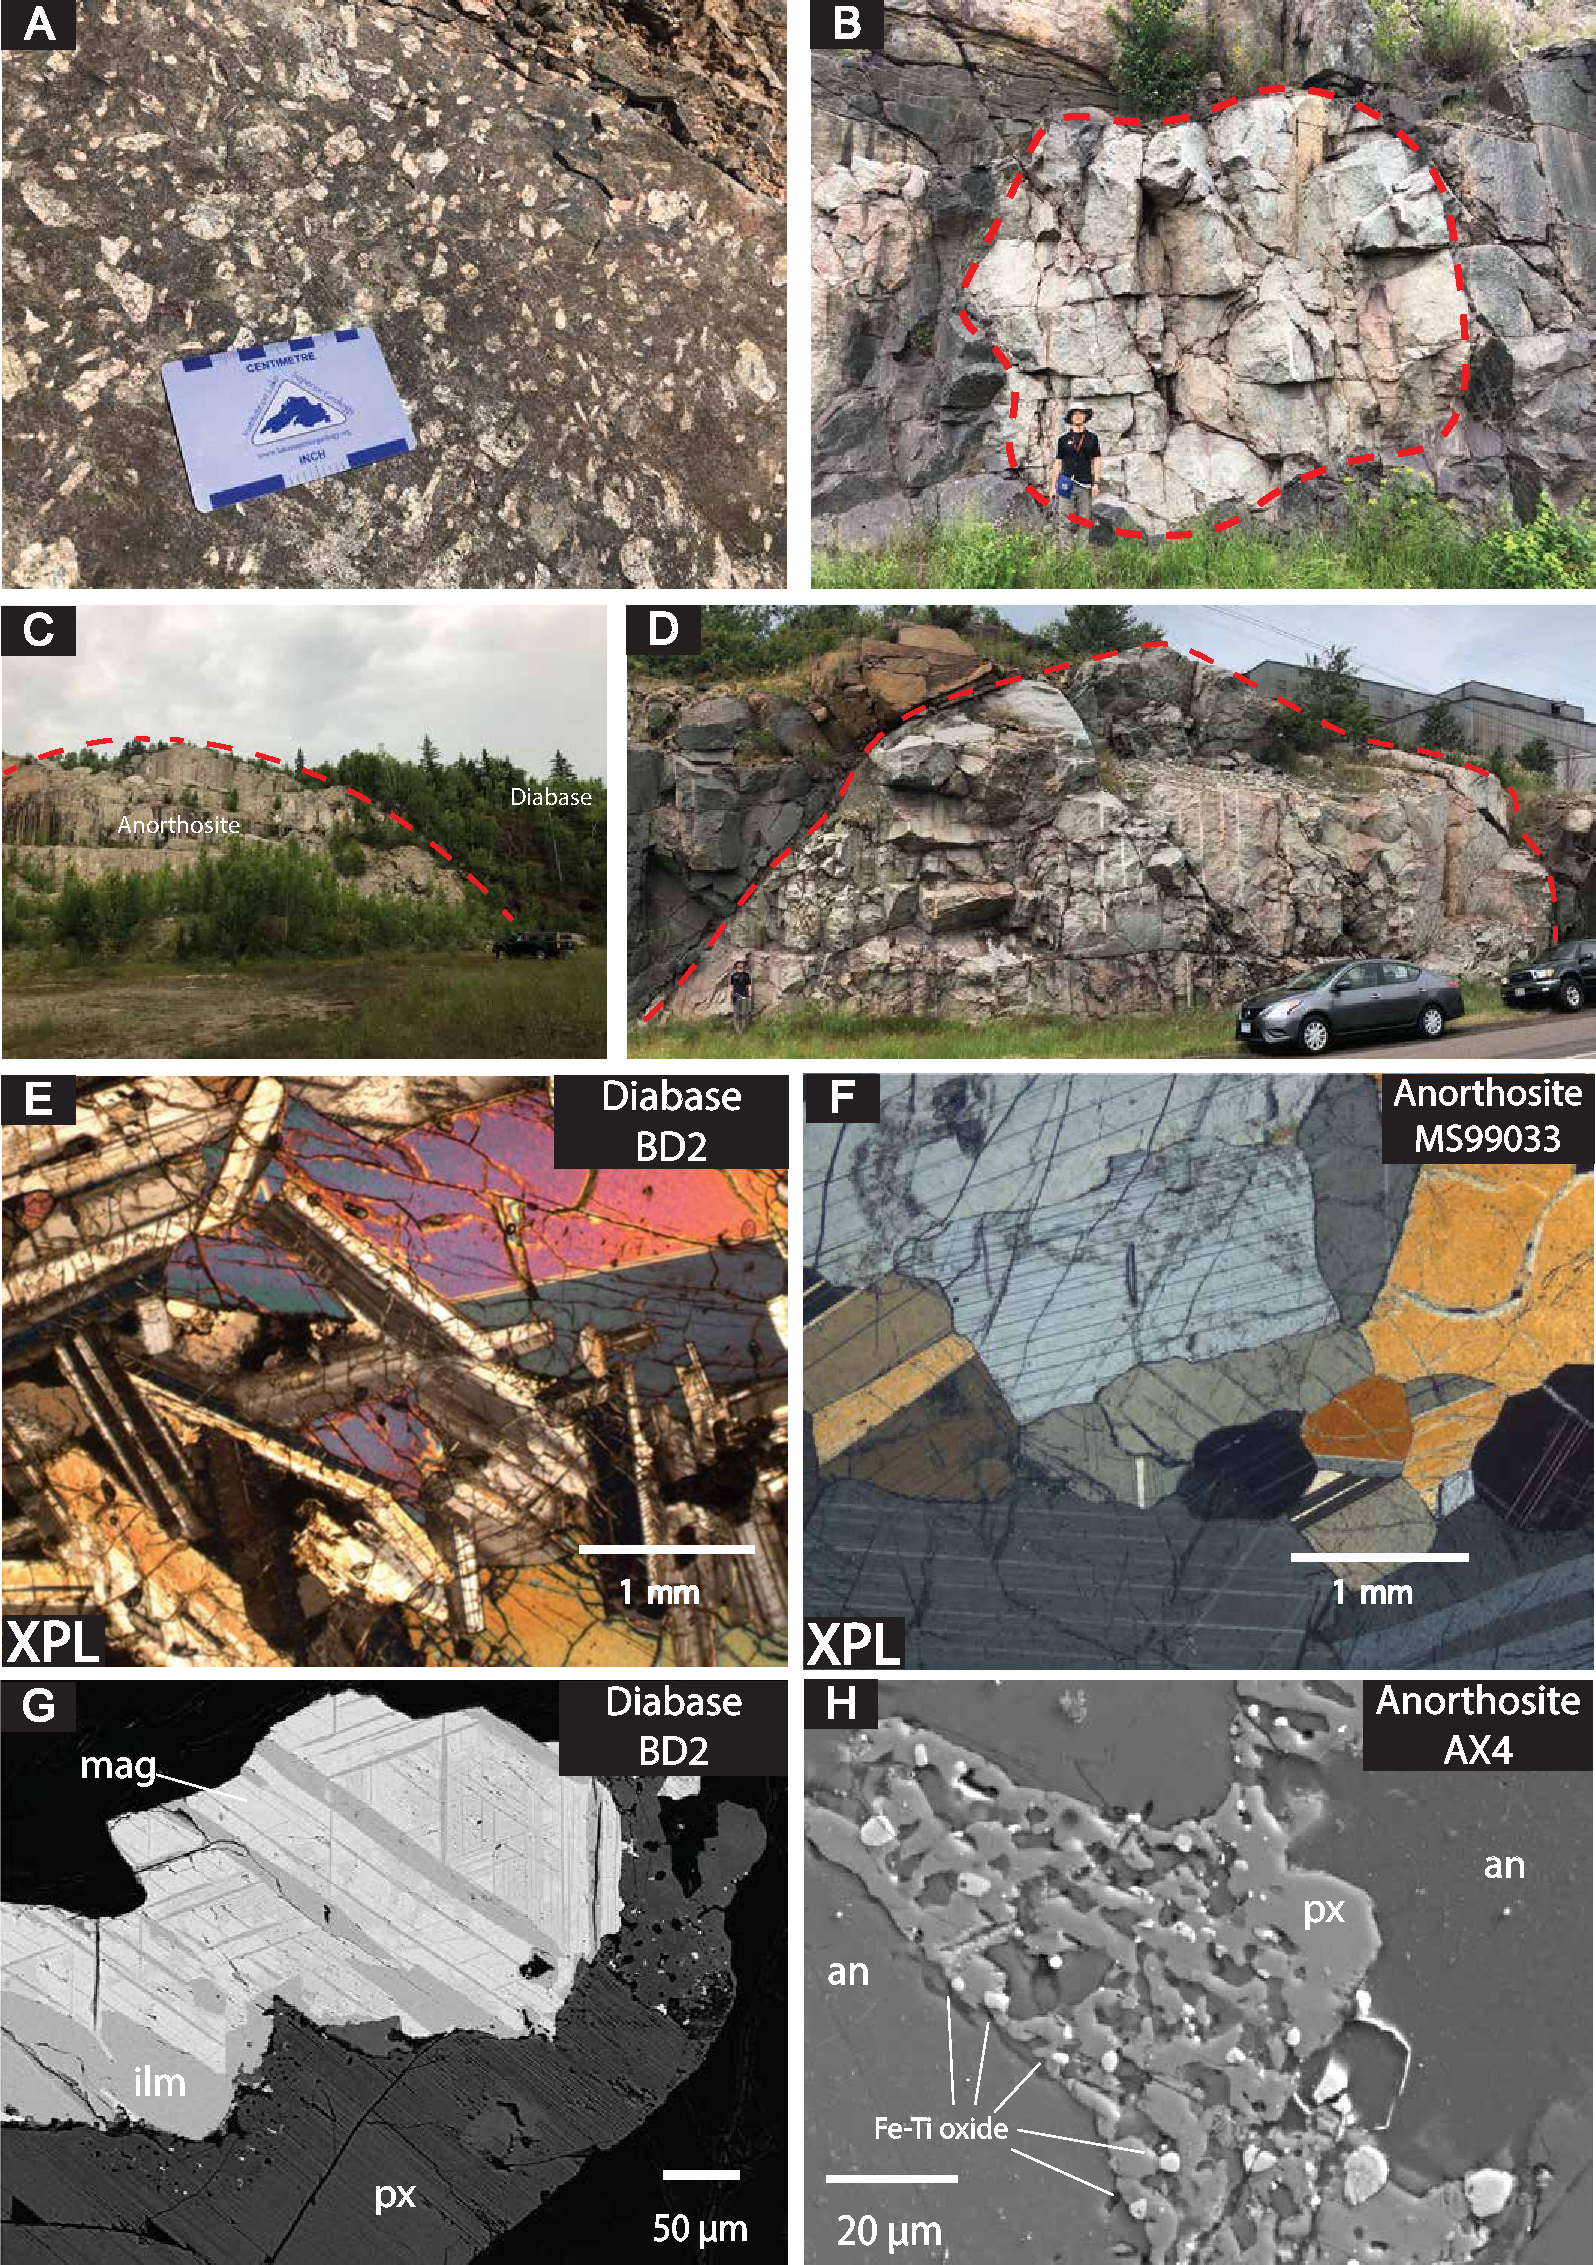
\includegraphics[width=0.8\textwidth]{figure/Zhang2024a/Field_photo.png}
\caption[Field photos of the Jacobsville Formation.]{\scriptsize Field photos of the Jacobsville Formation. (A) The red/white medium-grained sandstone with decimeter-scale trough cross-stratification in this image (taken at the shore near the unincorporated community of Jacobsville 46.9819\textdegree N, 88.4068\textdegree W) is a wide-spread lithofacies in the formation, but was not targeted for paleomagnetic sampling in this study. (B, C, D) At the Snake Creek tributary and the Natural Wall ravine in the northeastern Keweenaw Peninsula, intervals of red fine-grained sandstone to siltstone beds can be found through the steeply dipping to overturned basal strata near the Keweenaw fault and also the nearly horizontal upper strata. At the Dover Creek section (E), thick red siltstone horizons interbedded or interfingering with sandstones and conglomerates are found along a Dover Creek tributary waterfall (47.1708\textdegree N, 88.4466\textdegree W; this waterfall is distinct, but close to Hungarian Falls). Abundant reoriented siltstone intraclasts can be present within the conglomeratic layers above siltstone beds (Fig. \ref{fig:intraclast_pmag}). (F) At Agate Falls, nearly flat-lying red fissile siltstone beds are exposed. Detrital mica grains deposited parallel to the bedding plane are often present within the siltstone facies. Another set of siltstone intraclasts were sampled from a conglomeratic layer at Agate Falls for a paleomagnetic conglomerate test (Fig. \ref{fig:intraclast_pmag}).}
\label{fig:Field_photo}
\end{figure*}

The abundance of clasts of rift volcanics in the conglomeratic facies at Dover Creek, Hammel Creek, and Natural Wall indicates the presence of uplifted volcanics in proximity to the Keweenaw fault in the central part of the peninsula during Jacobsville deposition (Figs. \ref{fig:Chap_Jacobsville_Geologic_map} and \ref{fig:strat_column}). Coarse-grained arkosic to lithic sandstone is a facies associated with the volcanic-clast conglomerates and likely derived from mechanical weathering of the exhumed volcanics. Chemical weathering of exhumed volcanics from the hanging wall is a likely source of clay within the abundant fine-grained lithologies that are associated with the volcanic-clast conglomeratic facies (Fig. \ref{fig:strat_column}). Detrital zircon provenance data from Jacobsville samples on the Keweenaw Peninsula developed by \cite{Malone2020a} reveal zircon with dates overlapping with Midcontinent Rift volcanism consistent with this provenance interpretation.  Detrital mica grains up to $\sim$5 mm in size that are commonly found within siltstone to fine-grained sandstone within the Jacobsville are likely sourced from Paleoproterozoic and Archean lithologies in the region (Fig. \ref{fig:Chap_Jacobsville_Geologic_map}) and preferentially settled in lower energy overbank settings.

The thickness of the Jacobsville strata can vary in northern Michigan \citep{Hamblin1958a, Kalliokoski1982a}, and complete stratigraphic sections are not exposed at the studied localities (Figs. \ref{fig:Chap_Jacobsville_Geologic_map} and \ref{fig:strat_column}). Clay-rich red siltstone is more abundant in conjunction with conglomerates (e.g. 20-120 m in the Dover Creek section; Figs. \ref{fig:strat_column} and \ref{fig:Field_photo}) than with the cross-stratified sandstone which dominates much of the formation. Relatively thin lithic to arkosic sandstone beds, which are otherwise uncommon in the Jacobsville Formation, are commonly associated with the volcanic conglomerates and red siltstones near the Keweenaw fault (Fig. \ref{fig:strat_column}). Together, the volcanic conglomerates, red siltstones, and arkosic sandstones make up a unique facies association. As previously interpreted by \cite{Brojanigo1984a}, this facies association was likely deposited proximal to actively uplifting volcanic rocks near the Dover Creek, Hammel Creek, and Natural Wall sections (Fig. \ref{fig:strat_column}). The relative stratigraphic positions of the Agate Falls and Snake Creek tributary sections are less certain (Figs. \ref{fig:Chap_Jacobsville_Geologic_map} and \ref{fig:strat_column}).

The Jacobsville Formation has been mapped to have a continuous extent from the Wisconsin and Michigan border northeast to the Keweenaw Peninsula and east to the Marquette region (Fig. \ref{fig:Chap_Jacobsville_Geologic_map}; \citealp{Hamblin1958a, Cannon1995a, Cannon1996a, Cannon2001a}). In the eastern Lake Superior region near Sault Ste. Marie, Ontario, there are exposures of sedimentary rocks that are also mapped as the Jacobsville Formation \citep{Hamblin1958a}. As observed on the Keweenaw Peninsula, these sandstones are within the footwall of faults where they are overthrusted by Midcontinent Rift volcanics near Mamainse Point \citep{Manson1994a}. To the west, the Jacobsville Formation has been interpreted to be correlative with sedimentary rocks of the Bayfield Group in northern Wisconsin and the Fond du Lac Formation and Hinckley Formation in Minnesota \citep{Thwaites1912a, Hamblin1958a, Wallace1971a, Kalliokoski1982a, Ojakangas2001b}. A challenge associated with these correlations is that the ca. 1075 to 1050 Ma Freda Formation of the Oronto Group and the ca. 990 Ma Jacobsville Formation have quite similar fluvial lithofacies despite being deposited in distinct basinal settings at different times.

\section{Paleomagnetic results and interpretation}

Oriented paleomagnetic samples were collected with a portable electric drill from five stratigraphic sections of the Jacobsville Formation in northern Michigan (Figs. \ref{fig:Chap_Jacobsville_Geologic_map} and \ref{fig:strat_column}). Additional oriented cores and block samples of siltstone intraclasts within conglomerates and conglomeratic sandstones were sampled within the Dover Creek and Agate Falls sections (Figs. \ref{fig:Chap_Jacobsville_Geologic_map} and \ref{fig:strat_column}, and \ref{fig:intraclast_pmag}). To maximize sampling of distinct time snapshots of the geomagnetic field at the time of Jacobsville deposition and average out paleosecular variation, we optimized for vertical stratigraphic coverage \citep{Sapienza2023a}. Each sample is a distinct stratigraphic horizon and therefore a paleomagnetic site, representing a unique record of the geomagnetic field. Red fine-grained sandstone to shaly siltstone layers were preferentially sampled as they have lower permeability and are less susceptible to diagenetic alteration through fluid flow than coarser-grained sandstone. These fine-grained lithologies are typically of deep red color in contrast to coarse-grained lithologies that have splotchy tan, red, and light green coloration associated with secondary reduction (Fig. \ref{fig:Field_photo}A). Care was taken to avoid collecting samples with reduction spots. Paleomagnetic cores and blocks were oriented using a magnetic compass and a sun compass when possible. Sun compass data were preferentially used when available. A total of 379 specimens including 30 intraclasts were collected for paleomagnetic study. To minimize the visual impact of sampling, rock containing core holes was knocked out of outcrops following samples---readily done for the friable siltstones and sandstones of the Jacobsville Formation.

Challenges exist in isolating the primary magnetization in sedimentary rocks. Primary detrital remanence acquired during deposition can be masked by secondary remanence acquired through precipitation and growth of diagenetic minerals within sedimentary rocks syn- to post-deposition (e.g. pigmentary hematite formed from precursor phases such as ferrihydrite; \citealp{Jiang2018a}). In red beds, it has been found that formation of pigmentary hematite can post-date the timing of deposition, resulting in a chemical remanent magnetization superimposed upon primary detrital remanent magnetization carried by detrital grains \citep{Collinson1974a, Tauxe1980a}. To isolate the remanence components of sandstones of various grain sizes of the Jacobsville Formation, \cite{Roy1978a} adopted a method first applied by \cite{Collinson1965c} to preferentially remove fine-grained pigmentary hematite through prolonged immersion in concentrated HCl acid. Progressively longer immersion times first dissolve the nanometer-scale pigmentary hematite prior to dissolving the coarser micrometer-scale detrital grains. Studies applying paired acid etching demagnetization and thermal demagnetization show that the pigmentary hematite grains tend to have lower unblocking temperatures than detrital ones \citep{Tauxe1980a, Bilardello2010c}. High-resolution thermal demagnetization experiments with temperature intervals as small as 1-2 \textdegree C have also been shown to be effective in isolating detrital remanence from chemical remanence as coarser hematite grains tend to have higher unblocking temperatures closer to the N\'eel temperature of hematite \citep{Jiang2015a,Swanson-Hysell2019b}. 

In the Jacobsville Formation samples that we collected, there are both detrital hematite grains (10s of micrometers) as well as finer grained (sub-micrometer) pigmentary hematite (Fig. \ref{fig:SI_petrography}). We adopted a thermal demagnetization protocol with increasingly higher resolution approaching the N\'eel temperature of hematite (5 \textdegree C to 2 \textdegree C; Fig. \ref{fig:intraclast_pmag}, \ref{fig:SI_orthogonal}). The specimens underwent step-wise thermal demagnetization at the UC Berkeley Paleomagnetism Lab using an ASC demagnetizer (residual fields $<$10 nT) with measurements made on a 2G DC-SQUID magnetometer. Due to the thermal gradient in the oven, we keep the specimens at the same location throughout the demagnetization steps. This protocol makes the temperature difference between each step relatively consistent for each specimen compared to if they changed positions within the oven. While the very fine-grained sandstone and siltstone lithologies typically do not have an appreciable present-day local field overprint component, such a component can be present in fine-grained sandstones and is removed by $\sim$300\textdegree C during thermal demagnetization (Fig. \ref{fig:SI_orthogonal}, \ref{fig:Jacobsville_pdf}). A total of 356 specimens yielded detrital remanent magnetizations that can be fit with least-square lines \citep{Kirschvink1980a}. These fits were made using PmagPy \citep{Tauxe2016a} and all paleomagnetic data are available to the measurement level in the MagIC database (\url{https://doi. org/10.7288/V4/MAGIC/19780}).

\subsection{Paleomagnetic field tests}

\subsubsection{Fluvial intraclast conglomerate tests}

Similar to the thermal demagnetization results of the hematite-bearing fluvial intraclasts of the Freda Formation \citep{Swanson-Hysell2019b}, the siltstone intraclasts of the Jacobsville Formation typically reveal two distinct magnetization components (Fig. \ref{fig:intraclast_pmag}). One component shows similar vector orientations amongst intraclasts and was typically removed up to 640-655 \textdegree C (Fig. \ref{fig:intraclast_pmag}). The relatively low unblocking temperatures and similarity in directions among the reoriented intraclasts indicate that it is chemical remanent magnetization acquired through crystallization of secondary pigmentary hematite following clast redeposition. After removal of this component, further thermal demagnetization with small step increments at higher temperatures up to $\sim$689 \textdegree C often reveal an origin-trending component (Fig. \ref{fig:intraclast_pmag}). In the data from the clasts, there is typically a significant directional change in specimen magnetization between the mid-temperature component and the high-temperature component. As a result, 27 out of 30 intraclast specimens could be fit with high-temperature least squares lines. Distinct from the well-grouped mid-temperature component directions, the high-temperature directions of the intraclasts are dispersed and the null hypothesis of randomness cannot be rejected at the 95\% confidence level (n=5 for intraclasts at Agate Falls and n=22 for intraclasts at Dover Creek; Fig. \ref{fig:intraclast_pmag}; \citealp{Watson1956a}). This result indicates that the high unblocking temperature remanence is primary and was acquired by detrital hematite grains during initial deposition prior to the clasts being ripped up and reoriented within the depositional environment. This conglomerate test provides strong support for interpreting the high unblocking temperature remanence in the \textit{in situ} beds as a primary DRM. 

\begin{figure*}[h!]
\centering
\includegraphics[width=0.5\textwidth]{figure/Zhang2024a/intraclast_pmag.png}
\caption[Jacobsville Formation intraclast conglomerate test]{\scriptsize (A) Field photos of siltstone to fine-grained sandstone fluvial intraclasts within conglomerate and conglomeratic sandstone beds in the Jacobsville Formation. (B) Representative step-wise thermal demagnetization data from an intraclast from Dover Creek (HFC-23) plotted on an orthogonal vector diagram. The plot reveals a mid-temperature component and an origin-trending high-temperature component. The components are present as varying fractions of the overall remanence in different specimens. The direction of the mid-temperature component (interpreted as secondary CRM) is shown as dark red arrows on the orthogonal vector plots and dark red circles on the equal area plots, while the high-temperature component (interpreted as primary DRM) is shown in grey. (C, D) The mid-temperature component has a similar direction among the clasts as can be seen on the summary equal area plots. In contrast, the high-temperature component directions are dispersed and pass the randomness test of \cite{Watson1956a}. Both the DRM and the CRM directions are shown in geographic coordinates. NRM = natural remanent magnetization.}
\label{fig:intraclast_pmag}
\end{figure*}

\subsubsection{Fold test}

A total of 71 specimens yielded interpretable DRM directions throughout the stratigraphic section at the Snake Creek tributary (Figs. \ref{fig:Chap_Jacobsville_Geologic_map} and \ref{fig:in_situ_pmag}). The stratigraphic section is within a large-scale drag fold within the immediate footwall of the Keweenaw fault. As a result, there are exposures of steeply tilted, moderately tilted, as well as nearly horizontal beds along this section that allow us to conduct a paleomagnetic fold test to investigate the timing of magnetization. The chronological constraints on the timing of Keweenaw fault motion indicate that the folding occurred on a timescale of $\sim$10 Myr of deposition---making this fold test a more informative constraint on the age of the remanence than typical for such tests. Given that the more steeply tilted beds accommodated deformation during shortening associated with the Keweenaw fault motion, they could be more prone to non-cylindrical folding and complicate tilt-correction of the paleomagnetic directional data \cite[e.g.][]{Pueyo2003a, Nabavi2021a}. Therefore, we conduct a paleomagnetic bootstrap fold test \citep{Tauxe1994a} using specimens from the nearly horizontal beds and the moderately tilted beds. The results show that the degrees of untilting that result in the best grouping of the DRM directions have 95\% confidence bounds that overlap with 100\% unfolding, consistent with the specimens having acquired their magnetization prior to tilting (Fig. \ref{fig:fold_test}). This positive fold test further supports the interpretation that the Jacobsville red beds acquired a primary detrital remanence during deposition. In contrast, the mid-temperature component directions that typically unblock up to 650 \textdegree C from the Snake Creek tributary fails a fold test (Fig. \ref{fig:Jacobsville_hct_fold_test}), consistent with them being acquired as chemical remanent magnetizations that postdate the tilting. The positive fold test on the detrital remanence in combination with the similarity of the detrital and chemical remanence directions (Fig. 6B) indicates that the majority of chemical remanence acquisition likely occurred geologically soon after the deformation.

\begin{figure*}
\centering
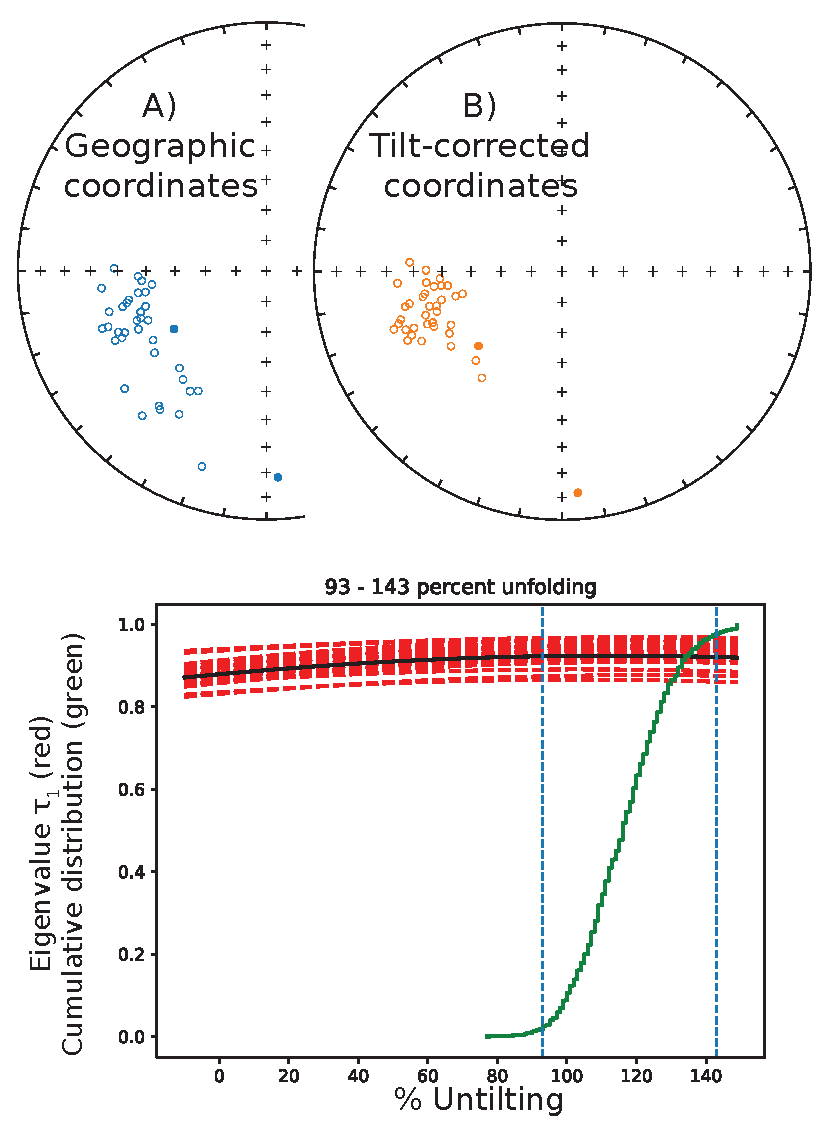
\includegraphics[width=0.6\textwidth]{figure/Zhang2024a/SC1_fold_test.pdf}
\caption[Jacobsville Formation fold test]{Bootstrap paleomagnetic fold test \citep{Tauxe1994a} of the detrital remanent magnetization directions recorded by specimens from the nearly horizontal beds and moderately tilted beds at the Snake Creek tributary. Complete unfolding lies within the 95\% confidence limits of the test, consistent with the magnetization having been acquired prior to tilting.}
\label{fig:fold_test}
\end{figure*}

\subsection{Paleomagnetic reversals}

With the insights gained from the thermal demagnetization results of the Jacobsville fluvial intraclasts and the fold test (Figs. \ref{fig:intraclast_pmag} and \ref{fig:fold_test}), we next investigate the detrital remanent magnetizations for all \textit{in situ} specimens from the five stratigraphic sections (Figs. \ref{fig:Chap_Jacobsville_Geologic_map} and \ref{fig:strat_column}). The DRM directions are plotted by stratigraphic section location in Figure \ref{fig:in_situ_pmag}. As observed in the sparser data of \cite{Roy1978a}, there are dual polarity magnetizations (Fig. \ref{fig:strat_column}). The paleomagnetic polarity reversals are shown in stratigraphic context in Figure \ref{fig:strat_column} with specimen magnetization declinations plotted against stratigraphic heights. The record of Laurentia's paleomagnetic poles from the Proterozoic through the Phanerozoic (see compilations in \cite{Torsvik2012a} and \cite{Swanson-Hysell2021c}) gives a continuity of the orientation of the continent that enables the geomagnetic polarity of the directions to be interpreted. In this framework, the westerly DRM directions are normal geomagnetic polarity and the easterly DRM directions are reversed polarity (Fig. \ref{fig:in_situ_pmag}). 

At the Dover Creek section, which goes along Dover Creek and then up the waterfall of a side tributary (the Hungarian Falls side falls), numerous hematite-rich siltstone to fine sandstone layers commonly occur in association with trough cross-bedded sandstone and conglomeratic facies. These lithofacies are particularly well-exposed along a tributary waterfall to Dover Creek such that 158 samples were collected for paleomagnetic study (Fig. \ref{fig:Chap_Jacobsville_Geologic_map}, \ref{fig:strat_column}), making this section the most densely sampled amongst all the sections. The specimen DRMs show that the geomagnetic field reversed at least nine times during deposition within the section (Fig. \ref{fig:strat_column}). 

The Natural Wall and Hammel Creek sections are in close proximity to the Dover Creek section (Fig. \ref{fig:Chap_Jacobsville_Geologic_map}) and the unique sedimentary facies association of volcanic-clast conglomerate, red siltstone, and coarse arkosic sandstone is similar to the basal $\sim$120 meters of the section at Dover Creek (Fig. \ref{fig:strat_column}). Our sampling at these two localities is more limited due to there being poorer exposures of siltstone and fine-grained sandstone beds in these sections (Fig. \ref{fig:strat_column}). At Hammel Creek, 16 samples from two siltstone layers near the base of the section are of reversed polarity (Fig. \ref{fig:strat_column}). Near the top of the Natural Wall section, consistent normal-polarity directions are recorded by 15 samples (Fig. \ref{fig:strat_column}). 

At the Snake Creek tributary (Fig. \ref{fig:Chap_Jacobsville_Geologic_map}), 71 specimens yielded interpretable DRMs through multiple levels along the $\sim$95-meter-thick section and all show normal-polarity directions (Figs. \ref{fig:in_situ_pmag} and \ref{fig:strat_column}). At Agate Falls (Fig. \ref{fig:Chap_Jacobsville_Geologic_map}), clay-rich detrital mica-bearing siltstone layers occur through $\sim$30 meters of strata that are incised by the Middle Branch Ontonagon River (Fig. \ref{fig:Field_photo}). 67 total paleomagnetic samples were collected on both sides of the waterfall (Fig. \ref{fig:strat_column}). At least three geomagnetic polarity reversals occurred during deposition within the Agate Falls section (Fig. \ref{fig:strat_column}). 

\begin{figure*}[h!]
\centering
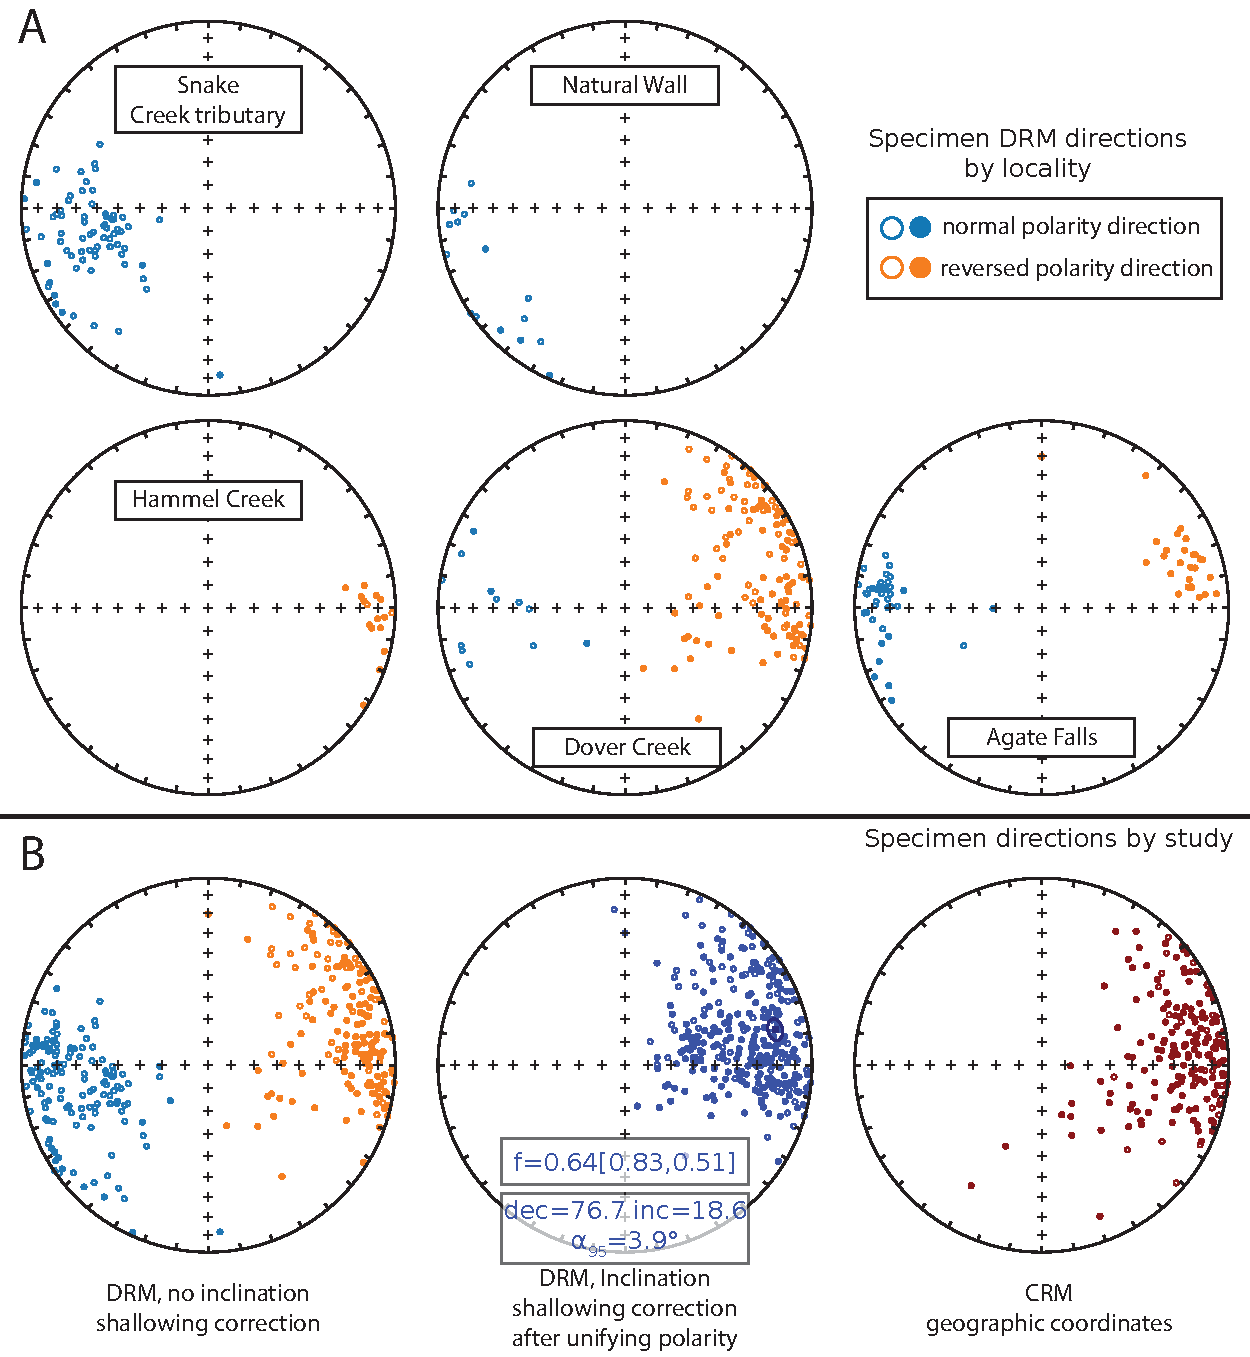
\includegraphics[width=0.78\textwidth]{figure/Zhang2024a/in_situ_pmag.pdf}
\caption[Summary figures for paleomagnetic results from the Jacobsville Formation]{\scriptsize (A) Specimen detrital remanence directions (DRM) plotted by locality on equal area plots. During sample collection, we optimized for vertical stratigraphic coverage such that each sample constitutes a single horizon and therefore a paleomagnetic site. Specimens from the Snake Creek tributary as a mean direction of dec=256.0\textdegree, inc=-30.5\textdegree, k=9.9, $\alpha_{95}$=5.6\textdegree, n=71; the Natural Wall section has a mean direction of dec=242.4\textdegree, inc=-6.4\textdegree, k=9.0, $\alpha_{95}$=13.5\textdegree, n=15; the Hammel Creek section has a mean direction of dec=94.1\textdegree, inc=8.7\textdegree, k=30.7, $\alpha_{95}$=6.8\textdegree, n=16; the Dover Creek section has a mean direction of dec=73.2\textdegree, inc=5.4\textdegree, k=5.6, $\alpha_{95}$=5.6\textdegree, n=138; the Agate Falls section has a mean direction of dec=83.4\textdegree, inc=13.0\textdegree, k=13.4, $\alpha_{95}$=4.9\textdegree, n=67. All reported directions are calculated in tilt-corrected coordinates and after unifying polarity. The measurement-level data are available in the MagIC database (\url{https://doi. org/10.7288/V4/MAGIC/19780}). (B) Summary equal area plots at the study-level combining directions from all localities. The elongation/inclination (E/I) method \citep{Tauxe2004b} was used to estimate the amount of inclination shallowing in Jacobsville specimen DRMs after unifying the polarities (flipping the normal [blue] directions to their antipodes). Details on inclination shallowing corrections are shown in Figure \ref{fig:EI_results} with the value of $f$=0.64 used for the directions in the middle panel. All DRM directions are shown in tilt-corrected bedding coordinates. The summary plot of all specimen chemical remanence directions (CRM) are shown in geographic coordinates show well-grouped reversed-polarity directions whose directions are similar to the DRMs. }
\label{fig:in_situ_pmag}
\end{figure*}

The paleomagnetic reversal test assesses whether two directional data sets share a common mean when one of the polarity directions is flipped to its antipode. Although the occurrence of multiple geomagnetic field reversals during deposition of the Jacobsville Formation is evident (Figs. \ref{fig:strat_column} and \ref{fig:in_situ_pmag}), the limited and often discrete records of many polarity chrons are insufficient for pair-wise reversal tests within single sections (Fig. \ref{fig:strat_column}). Sedimentation within individual siltstone horizons was likely quite rapid given their deposition within fluvial floodplains potentially without sufficient time to average out secular variation within discrete siltstone intervals. We combine all normal and reversed directions from the five sections and perform a reversal test. The \cite{McFadden1990a} reversal test results show the angle between the two mean directions (15.9\textdegree; no inclination shallowing correction) exceeds the critical angle (7.5\textdegree) (Fig. \ref{fig:Jacobsville_reversal_test}), thereby failing the test. This difference largely arises due to normal (west directed) directions in the Snake Creek tributary section being slightly steeper in their upward inclination. There are at least four possible explanations for this behavior: 1) the lower number of normal directions which dominantly come from the Snake Creek tributary section may not have averaged out secular variation; 2) there could have been plate motion during Jacobsville deposition with the normal polarity in the Snake Creek tributary section being acquired when Laurentia was at a slightly higher latitude; 3) there could be a bias from the reversed CRM superimposed on the normal DRM in the Snake Creek tributary specimens being incompletely removed during thermal demagnetization; 4) the geomagnetic field in the early Neoproterozoic could have been slightly different than that of more recent times in terms of the dispersion of pole position at distinct time snapshots potentially associated with changes in field intensity. Regardless, the positive intraclast conglomerate test gives confidence that the Jacobsville Formation has a primary detrital remanent magnetization that can be isolated through thermal demagnetization. This result is strengthened through the positive fold test and the broadly antipodal dual polarity data. Additionally, taking the large number of samples together from both polarities to calculate a pole increases the likelihood that the dual polarity pole has averaged out secular variation.

A total of 186 specimens yielded interpretable chemical remanence directions that are of dominantly reversed polarity. These directions are plotted by stratigraphic section location in Figure \ref{fig:Jacobsville_CRM} and are all shown in Figure 6B. That the CRM directions are a secondary remanence component that postdate the deposition of the Jacobsville Formation is supported by the negative intraformational conglomerate test results and failure in the fold test (Figs. \ref{fig:intraclast_pmag}, S4). However, the similarity of the CRM directions (declination=96.2\textdegree, inclination=15.1\textdegree, $\alpha_{95}$=4.2\textdegree, n=186) with the primary DRM directions (declination=76.9\textdegree, inclination=13.4\textdegree, $\alpha_{95}$=3.3\textdegree, n=307, no inclination shallowing correction) indicate that growth of the secondary pigmentary hematite which carries the CRM likely occurred soon after deposition when Laurentia was in a similar paleogeographic position. 

Overall, the multiple geomagnetic field polarity reversals recorded by the Jacobsville Formation constrain that the end of the Keweenawan normal superchron \citep{Driscoll2016b} (which started ca. 1099 Ma; \citealp{Swanson-Hysell2019a}) had to have ended by the onset of Jacobsville deposition.
 
\section{Discussion}
\subsection{Averaging paleosecular variation and correcting for inclination shallowing}

Igneous and sedimentary rocks associated with the North American Midcontinent Rift provide a high-resolution record of the ca. 1109 to 1070 Ma Keweenawan Track which tightly constrains the apparent polar wander path for Laurentia in the late Mesoproterozoic (Fig. \ref{fig:pole_plot}; \citealp{Swanson-Hysell2019a}). However, high-quality paleogeographic constraints thereafter are sparser and more uncertain in their age until the ca. 775 Ma Gunbarrel large igneous province \citep{Harlan2003a} and subsequent ca. 775-719 Ma poles from western Laurentia extensional basins \citep{Weil2006a, Eyster2019a}. Developing a new paleomagnetic pole from the Jacobsville Formation presents an opportunity for a well-constrained early Neoproterozoic constraint on Laurentia's paleogeographic position. 

Our high-resolution thermal demagnetization successfully isolated detrital magnetization from the secondary chemical magnetization carried by pigmentary hematite that grew after deposition of the Jacobsville Formation. The scatter in the DRM directions can be interpreted to reflect variations in the geomagnetic field during the deposition of the sediments \citep{Steiner1983a, Tauxe1984a}. The multiple geomagnetic field reversals captured by specimens collected from the Dover Creek and Agate Falls sections support that a prolonged period of time is represented by the specimens given that the duration of geomagnetic polarity chrons are typically on the order of tens of Kyr to Myr timescales (Fig. \ref{fig:strat_column}). Therefore, we combine all specimen detrital remanent magnetizations to calculate a paleomagnetic pole for the Jacobsville Formation.

A challenge in interpreting detrital magnetizations is the issue of correcting for inclination shallowing \citep{King1955a, Tauxe2004b, Bilardello2016b}. Scatter of the specimen detrital remanence directions in tilt-corrected coordinates show elongation parallel to the bedding plane, consistent with them being shallowed (Fig. \ref{fig:in_situ_pmag}; \citealp{Tauxe2004b}). Such a directional distribution is due to rotation of detrital hematite grains during deposition and subsequent compaction, resulting in inclinations recorded by sedimentary rocks having shallower angles than the local field in which they are deposited. If uncorrected, shallower inclinations obtained from sedimentary rocks can result in erroneously low estimates of paleolatitudes, biasing paleogeographic reconstructions. To estimate the amount of inclination shallowing, we apply the statistical elongation/inclination (E/I) method that evaluates the deviation of the distribution of a large number ($>$100) of observed sedimentary paleomagnetic directional data with the predicted distribution given by a statistical paleosecular variation model \citep{Tauxe2004b}. Although the TK03 paleosecular variation model is based on data of relatively recent geomagnetic field variations, it has been shown to be compatible with data from the ca. 1.1 Ga lava flows of the Midcontinent Rift \citep{Tauxe2009a}. Furthermore, \cite{Pierce2022a} showed that applying the E/I method to detrital hematite magnetizations within the ca. 1093 Ma Cut Face Creek Sandstone in the Midcontinent Rift successfully corrects the shallow paleomagnetic inclinations of the sediments to that of the North Shore Volcanic Group lava flows that bracket them. \cite{Pierce2022a} also developed a method, that we use here, to represent uncertainties associated with the amount of inclination shallowing into sedimentary paleomagnetic pole positions which can then be summarized with an elliptical Kent distribution \citep{Kent1982a} rather than a circular Fisher distribution \citep{Fisher1953a}. 

Applying the E/I method to the Jacobsville DRM directions results in an estimate for the flattening factor ($f$ factor) of 0.64 with a 95\% uncertainty range of 0.83 to 0.51 (Figs. \ref{fig:EI_results}). The $f$ factor of 0.64 is close to the value of 0.58 which is the mean of inclination shallowing factors compiled for hematite-bearing rocks in \cite{Pierce2022a} (building on compilations of \cite{Bilardello2016b} and \cite{Vaes2021a}). The Fisher mean inclination-corrected detrital remanence mean direction is dec=76.7\textdegree, inc=18.6\textdegree $\alpha_{95}$=3.9\textdegree. The Fisher mean inclination-corrected paleomagnetic pole associated with this nominal $f$ factor is Plon=183.4\textdegree E, Plat=16.9\textdegree S, A$_{95}$=3.1\textdegree. We apply the method of \cite{Pierce2022a} to incorporate the uncertainty in the E/I estimate of the $f$ factor into the uncertainty of the paleomagnetic pole (Fig. \ref{fig:EI_results}). This uncertainty results in more uncertainty associated with paleolatitude which for the pole is along the great circle path between the mean pole position and the locality of the Jacobsville sections. Following \cite{Pierce2022a}, the pole can be represented with a Kent distribution 95\% confidence ellipse which is: mean longitude=183.4\textdegree E, mean latitude=16.9\textdegree S, major axis longitude=255.5\textdegree E, major axis latitude=45.2\textdegree N, major axis magnitude=4.1\textdegree, minor axis longitude=108.1\textdegree E, minor axis latitude=39.9\textdegree N, minor axis magnitude=3.1\textdegree (Fig. \ref{fig:EI_results}; Table \ref{tab:Kent_means}). This pole position is close to the end of the Keweenawan Track (Fig.\ref{fig:pole_plot}) and far away from Laurentia's pole positions during the Paleozoic when there was orogenesis along Laurentia's eastern margin (Fig. \ref{fig:Jacobsville_Appalachian}). This pole position is consistent with the geochronology constraints on the deposition of the Jacobsville Formation and the positive paleomagnetic field tests that the detrital remanence of the Jacobsville Formation was acquired during the earliest Neoproterozoic. 


\begin{figure*}[h!]
\centering
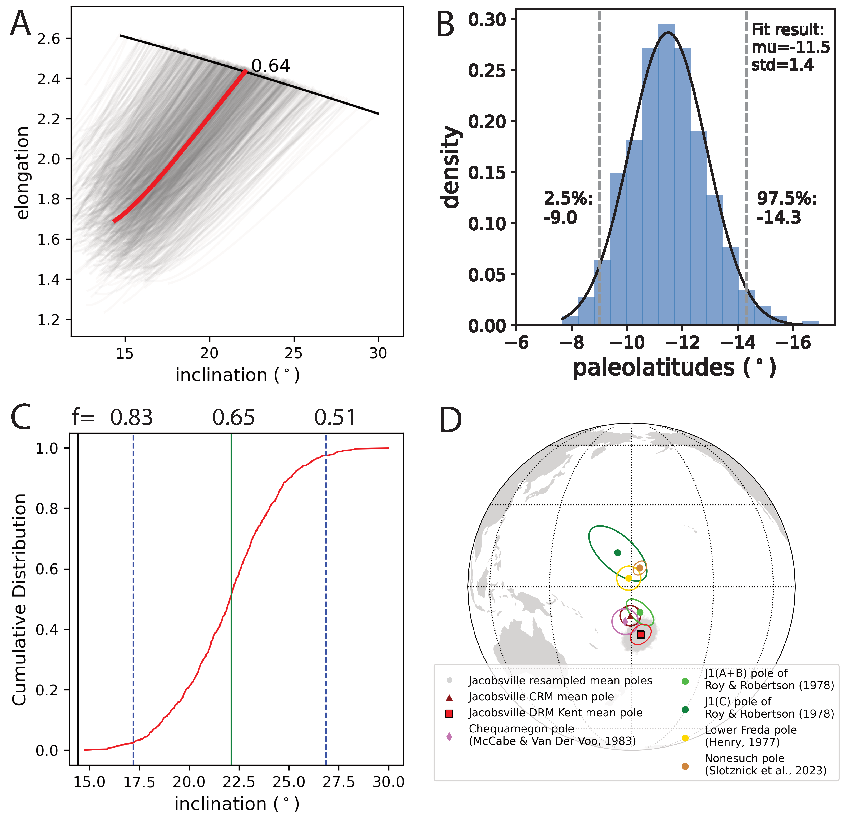
\includegraphics[width=0.8\textwidth]{figure/Zhang2024a/EI_results.pdf}
\caption[Jacobsville Formation inclination shallowing correction]{\scriptsize Results of the estimated amount of inclination shallowing of the detrital remanent magnetization of the Jacobsville Formation using the elongation/inclination (E/I) method \citep{Tauxe2004b}. (A) The E/I method gives an estimated flattening factor $f$=0.64 (red curve) based on where the elongation/inclination curve of the dataset intersects that predicted by the TK03 paleosecular variation model (black curve; \citealp{Tauxe2004b}). The grey lines show 1,000 bootstrap resamples of the DRM directions which provide an estimate of the uncertainty associated with the $f$ factor estimate (95\% interval from 0.83 to 0.51). (B) The distribution of the paleolatitudes resulting from the corrected inclinations of the E/I bootstrap resamples. That the distribution is drawn from a normal distribution with a mean of -11.5\textdegree\ and standard deviation of 1.4 cannot be rejected in the Kolmogorov-Smirnov test. The 95\% confidence bounds shown by dashed lines span a range of paleolatitudes that need to be incorporated into the uncertainty of the reported paleomagnetic pole. (C) The cumulative distribution of inclinations based on the E/I bootstrap results with the 95\% confidence bounds shown in terms of inclination and $f$ factor. (D) The new Kent mean inclination corrected DRM pole (red square) of the Jacobsville Formation is shown in the context of the pole calculated for the CRM (purple triangle) as well as the Jacobsville pole developed by \cite{Roy1978a}, the Chequamegon Formation pole of \cite{McCabe1983a}, and poles from the Oronto Group (Nonesuch Formation, \citealp{Slotznick2023a}; Freda Formation, \citealp{Henry1977a}). The mean pole position of the Kent distribution was calculated following the method of \cite{Pierce2022a}. The close proximity between Jacobsville poles with the Chequamegon pole is consistent with their deposition being coeval. In contrast, the J1 (C) pole of \cite{Roy1978a} developed from hematite-bearing sedimentary rocks in the Sault Ste Marie region plots in the northern hemisphere close to the Freda Formation pole. }
\label{fig:EI_results}
\end{figure*}

\begin{table}[h!]
   \caption{Kent mean paleomagnetic pole for the Jacobsville Formation} 
   \label{tab:Kent_means}
   \footnotesize
   \centering
   \begin{tabular}{p{0.8 in}p{0.8 in}p{0.8 in}p{0.8 in}p{0.8 in}p{0.8 in}}
   \hline
   pole & mean pole position (Plon/Plat) & major axis & major axis 95\% confidence angle & minor axis & minor axis 95\% confidence angle \\
   & $\gamma_{1}$ & $\gamma_{2}$ & $\zeta_{95}$ & $\gamma_{3}$ & $\eta_{95}$ \\
   \hline
   Jacobsville $E/I$ corrected & 183.4\textdegree E / 16.9\textdegree S &  255.5\textdegree E / 45.2\textdegree N & 4.1\textdegree &
   108.1\textdegree E / 39.9\textdegree N & 3.1\textdegree \\
   \hline
 \multicolumn{6}{p{5.5 in}}{Notes: The Fisher mean of the Jacobsville detrital remanence paleomagnetic pole without an inclination shallowing correction is Plon=185.5\textdegree E, Plat=14.0\textdegree S, A$_{95}$=2.7\textdegree; the Fisher mean of the Jacobsville detrital remanence paleomagnetic pole with an inclination shallowing correction of $f$=0.64 is Plon=183.4\textdegree E, Plat=16.9\textdegree S, A$_{95}$=3.1\textdegree; the Fisher mean of the Jacobsville chemical remanence paleomagnetic pole is Plon=179.6\textdegree E, Plat=10.2\textdegree S, A$_{95}$=3.6\textdegree\.}
   \end{tabular}
\end{table}

\cite{Roy1978a} also studied the paleomagnetism of sedimentary rocks grouped as the Jacobsville Formation and isolated a characteristic magnetization component via alternating-field, thermal, and chemical demagnetization on a suite of Jacobsville red beds near the Keweenaw Peninsula (their area A), the town of Marquette (their area B), and Sault Ste Marie (their area C). Although least-squares principal component analyses was not a routine approach in fitting paleomagnetic directions at the time, that study had success in removing the present day local field overprint and was able to resolve dual magnetic polarities at one locality. The mean paleomagnetic pole position calculated from the interpreted primary magnetic remanence from rocks of the Keweenaw Peninsula and Marquette area (J1 A+B pole; pole longitude=183\textdegree E, pole latitude=9\textdegree S, dp=3\textdegree, dm=6\textdegree; no inclination correction; Fig. \ref{fig:EI_results}; \citealp{Roy1978a}) is in the southern hemisphere and lies close to the mean pole from this study (Fig. \ref{fig:EI_results}). However, their mean pole developed from fine- and medium-grained sandstone near Sault Ste Marie lies in the northern hemisphere with a pole latitude of 12\textdegree N (Fig. \ref{fig:EI_results}). Despite the large uncertainty ellipse associated with this mean pole position, it is distinct from the mean pole position from the Jacobsville Formation in northern Michigan. Instead, it overlaps with the Oronto Group paleomagnetic poles of the ca. 1070 Ma lower Freda Formation and the ca. 1075 Ma Nonesuch Formation (Fig. \ref{fig:EI_results}; \citealp{Henry1977a, Slotznick2023a}). As suggested by \cite{Dubois1962a} and \cite{Roy1978a}, these data suggest that the fluvial red beds in the Sault Ste Marie area that are often taken to be correlative to the Jacobsville Formation \cite[e.g.][]{Malone2020a} are likely time equivalent to sedimentary rocks of the Oronto Group and deposited during post-rift thermal subsidence. 

Deposition of Bayfield Group sedimentary rocks in northern Wisconsin (west of the studied exposures; Fig. \ref{fig:Chap_Jacobsville_Geologic_map}) has been hypothesized to be coeval with the Jacobsville Formation \citep{Hamblin1958a, Kalliokoski1982a, Malone2016a}. Published low precision detrital zircon U-Pb dates developed by laser ablation–inductively coupled plasma–mass spectrometry (LA-ICP-MS) dates are consistent with this interpretation with a maximum depositional age of ca. 1035 Ma for the Chequamegon Formation of the Bayfield Group \citep{Craddock2013a}. Our updated Jacobsville pole position is close to a pole developed from the Chequamegon Sandstone of the Bayfield Group (Fig. \ref{fig:EI_results}; pole longitude=177.7\textdegree E, pole latitude=12.3\textdegree S, A$_95$=4.6\textdegree; no inclination correction; \citealp{McCabe1983a}). These data are consistent with the Bayfield Group being deposited within a contiguous syn-orogenic basin with the Jacobsville Formation during the Rigolet phase of the Grenvillian orogeny. This interpretation can be evaluated with further high-precision geochronology focused on the Bayfield Group. 

\subsection{Age of the Jacobsville Pole}

At the western edge of the Jacobsville bedrock belt in northern Michigan, the formation is in angular unconformity with Midcontinent Rift rocks that were uplifted and tilted prior to Jacobsville deposition (Fig. \ref{fig:Chap_Jacobsville_Geologic_map}; \citealp{Hedgman1992a, Cannon1995a}). Rb-Sr thermochronologic data developed from Paleoproterozoic to Archean lithologies that were exhumed along the Marenisco Fault along with Midcontinent Rift strata in this region indicate that this uplift occurred ca. 1050 Ma associated with the Ottawan phase of the Grenvillian orogeny \citep{Cannon1993a}. Field observations reveal erosional contacts and development of paleosols between the Jacobsville Formation and underlying Midcontinent Rift volcanic rocks at the Sturgeon River within the bedrock belt \citep{Hamblin1958a, Zbinden1988a}. Seismic reflection data beneath Lake Superior have been also been interpreted to indicate that the Jacobsville Formation lies in angular unconformity atop sedimentary rocks of the Oronto Group \citep{Cannon1989a}. This context requires that there was ca. 1050 Ma contractional deformation of Midcontinent Rift strata, erosion of these tilted strata, and renewed subsidence prior to the onset of Jacobsville deposition atop them.

Maximum depositional detrital zircon dates are consistent with this history and provide additional constraints. \cite{Hodgin2022a} applied tandem dating where the young population emerging from a large number of low-precision LA-ICP-MS dates are followed by high-precision CA-ID-TIMS analysis. This approach has the advantage of combining the high number of low-precision analyses that can be acquired through LA-ICP-MS with dates developed through CA-ID-TIMS where the deleterious effects of Pb-loss can be mitigated, and more accurate and precise dates can be obtained. These data reveal the youngest zircon at Sandstone Creek near the Keweenaw fault (Figure \ref{fig:Chap_Jacobsville_Geologic_map}) to have a date of 992.51 $\pm$ 0.64 Ma (2$\sigma$ analytical uncertainty) and the youngest zircon at Agate Falls (Figure \ref{fig:Chap_Jacobsville_Geologic_map}) a date of 1003.21 $\pm$ 2.23 Ma (2$\sigma$). These dates are consistent with the age of syntectonic magmatism in the Grenville orogen associated with the Rigolet phase of the orogeny \cite[e.g.][]{Bussy1995a, Turlin2019a, Jannin2018a} which is a potential source for the grains. Overall, these dates constrain a maximum depositional age of the Jacobsville Formation in the earliest Neoproterozoic. 

While there has been recent success in applying tandem detrital zircon data to obtain maximum depositional ages that are close to true depositional ages \citep{Karlstrom2020a}, the possibility exists that deposition could significantly postdate the youngest dated detrital zircon. A firm minimum depositional age on the age of the Jacobsville is that it is unconformably overlain by the Cambrian Munising Formation whose base was deposited ca. 501 to 497 Ma during the Dresbachian Stage (the Guzhangian Stage in the modern Cambrian time scale) \citep{Hamblin1958a, Haddox1990a}. This unconformity is erosional as it truncates Jacobsville strata and intraformational clastic dikes and can have slight angularity \citep{Hamblin1958a, Haddox1990a}. That the Jacobsville Formation is older than the Munising Formation lends tighter constraints than the Cambrian age itself given the evidence discussed above that Jacobsville deposition was syn-orogenic. The only candidate for such orogenesis is the ca. 1010-980 Ma Rigolet phase of the Grenvillian orogeny given that subsequent Paleozoic orogenesis (e.g. the Ordovician Taconic and Carboniferous Alleghanian orogenies) post-dates deposition of the Munising Formation.

That the Jacobsville Formation is folded in the footwall of the Keweenaw fault, beneath the older Midcontinent Rift volcanic rocks in the hanging wall, provides another opportunity to develop a minimum depositional age. Seeking to obtain such a constraint, \cite{Hodgin2022a} targeted calcite within a Keweenaw fault breccia that cross-cuts a dense network of zeolite veins and slickenslides that yielded a U-Pb date of 985.5 $\pm$ 35.8 Ma (2$\sigma$). While this calcite date has large analytical uncertainty, it indicates that the fault breccia developed associated with the Grenvillian orogeny and it overlaps with the ca. 1010-980 Ma ages of metamorphism associated with the Rigolet phase of the orogeny \citep{Swanson-Hysell2023a}. It is during this ca. 1010-980 Ma Rigolet phase of the orogeny that the Grenville Front developed \citep{Rivers2008a} which indicates that this was a time period when contractional deformation associated with the orogeny was propagating into the Superior craton. Together, the detrital zircon, sedimentology, and the fault calcite dates are consistent with the Jacobsville Formation being deposited in a syn-orogenic Grenville backbulge basin and subsequently deformed as contraction associated with the Rigolet phase of the Grenville orogeny propagated into the interior of Laurentia. 

Previously, some researchers have interpreted there to have been large-scale regional contractional deformation during the Alleghanian orogeny in the Paleozoic leading to reactivation of reverse faults including the Keweenaw fault \citep{Craddock2017a}. While the Keweenaw fault is defined quite broadly in \cite{Craddock2017a}, the evidence put forward that is relevant to the segment in this study region are: 1) an interpreted post-Grenvillian orogeny age for the Jacobsville Formation which would require that the deformation of the formation was associated with subsequent orogenesis; and 2) deformation within two $<$1.5 km diameter outliers of Paleozoic sedimentary rocks that overlie the Jacobsville (Limestone Mountain in Figure \ref{fig:Chap_Jacobsville_Geologic_map}). The data used to argue for a post-Grenvillian depositional age of the Jacobsville Formation were the low-precision LA-ICP-MS detrital zircon dates of \cite{Malone2016a} that have now been superseded by the tandem dates of \cite{Hodgin2022a}. These dates are consistent with syn-Grenvillian deposition. This progress leaves the tilted and/or brecciated Paleozoic strata in the small exposed Paleozoic outliers of the 1.5 x 1 km Limestone Mountain and the neighboring 0.5 x 0.3 km Sherman Hill as evidence of Paleozoic deformation: interpreted to be Paleozoic orogenesis by \cite{Hamblin1958a} and \cite{Craddock2017a} and suggested to be an impact structure by others \citep{Milstein1987a}. The impact origin interpretation builds on previous interpretations of the structure as being cryptovolcanic \citep{Cannon1981a}--a common interpretation for structures that have subsequently been recognized as impact related. The tilt and brecciation of these outliers contrasts with widespread flat-laying Paleozoic sedimentary rocks that overlie the reverse faults that underwent contractional deformation associated with rift inversion in Minnesota \citep{Jirsa2011a}. These strata constrain Paleozoic deformation to have been relatively minor on the scale of 10s of meters rather than the kilometers of uplift associated with the rift inversion along these reverse faults \citep{Boerboom2018a}. Clumped isotope temperatures of $\sim$50\textdegree C from the Neoproterozoic fault calcite, also developed by \cite{Hodgin2022a}, reveal that the Keweenaw fault zone was within a couple kilometers of the surface at the time of late Mesoproterozoic to early Neoproterozoic calcite precipitation. These data are inconsistent with major Paleozoic uplift and support the interpretation that the majority of contractional inversion along the Keweenaw fault occurred during the Rigolet Stage of the orogeny. 

Our new paleomagnetic data provide additional insights into the timing of Jacobsville deformation in the early Neoproterozoic. At the Snake Creek tributary section which is folded against the Keweenaw fault (Figure \ref{fig:Chap_Jacobsville_Geologic_map}, \ref{fig:strat_column}), the chemical remanence directions held by pigmentary hematite fail a fold test (Figure \ref{fig:Jacobsville_hct_fold_test}), indicating that the pigmentary hematite holding the remanence grew after deformation of the strata. The mean pole position of the chemical remanent magnetization at the Snake Creek tributary section overlaps with paleomagnetic poles of the Grenville Loop that have been assigned exhumation ages of ca. 970-960 Ma (Figure \ref{fig:Jacobsville_Appalachian}; \citealp{Brown2012a}). This chemical remanence pole position and the mean Jacobsville detrital remanence pole position are both far away from Laurentia's pole positions at the times of Paleozoic orogenesis or any younger time in the Phanerozoic (Figure \ref{fig:Jacobsville_Appalachian}). This result indicates that the majority of the tilting of the Jacobsville in the footwall of the Keweenaw fault could not have occurred during Paleozoic orogenesis such as the Alleghanian orogeny as the chemical remanent magnetization would then be expected to record a direction aligned with the Phanerozoic pole path. Instead, the Rigolet phase of Grenvillian orogeny, which ended by ca. 980 Ma, is the only feasible orogenic interval that could have tilted these strata. This result constrains the Jacobsville Formation in the studied outcrop belt to have been deposited prior to ca. 980 Ma. While Paleozoic reactivation could have occurred, and there could be deformation of that age elsewhere such as at Limestone Mountain, deformation at this time on the Keweenaw fault would have been relatively minor compared to that in the early Neoproterozoic.

In conclusion, our paleomagnetic data and existing chronological data combined with the geological constraints are most consistent with the interpretation that the Jacobsville Formation within the studied bedrock belt was deposited in a syn-orogenic basin associated with the Rigolet Phase of the Grenvillian orogeny. This syn-orogenic basinal setting, which is consistent with the sedimentology of the formation (Fig. \ref{fig:strat_column}), provides a mechanism for developing accommodation space. The total duration of deposition of the Jacobsville is uncertain with these constraints alone particularly given the low precision on the 985.5 $\pm$ 35.8 Ma calcite date. However, data from the Grenville orogen itself constrain the end of the Rigolet phase to be ca. 980 Ma \citep{Swanson-Hysell2023a}. As the studied sections proximal to the Keweenaw fault were deformed in its footwall during this phase of contractional deformation, it is reasonable to interpret deposition as occurring before the ca. 980 Ma cessation of Grenvillian orogenesis. Taken together, we consider the best nominal age constraint for the depositional age of the Jacobsville Formation to pair with the Jacobsville paleomagnetic pole position to be ca. 990 Ma as the Rigolet phase of the orogeny was ongoing. While deposition within peripheral foreland basins typically lasts between 10 and 50 million years \citep{Woodcock2004a}, the backbulge depocenter may not be as stable or long-lived. Given the available chronometric constraints from the Jacobsville Formation, the Keweenaw fault and the Rigolet phase in the Grenville orogen, deposition of the Jacobsville can be considered to have occurred within the 1000 to 980 Ma time interval.

\subsection{Slowdown of Laurentia's plate motion due to the Grenvillian orogeny}

The ca. 1109-1070 Ma Keweenawan Track constrains rapid motion of Laurentia from high latitudes toward the equator (Fig. \ref{fig:Jacobsville_paleogeography}; \citealp{Davis1997a, Swanson-Hysell2019a}). Apparent polar wander path inversion results are consistent with the pole path being dominated by plate tectonic motion that could have reached a rate of 30 cm/yr (95\% interval of 27-34 cm/yr; one Euler pole scenario; \citealp{Swanson-Hysell2019a, Rose2022a}); even faster than the rate of Indian plate motion during the closure of the Neotethys Ocean \citep{Hinsbergen2022a, Jagoutz2015a}. Laurentia's rapid motion preceded and coincided with the onset of the collisional Grenvillian orogeny. In contrast to the rapid changes in pole position associated with the Keweenawan Track, the relatively close proximity between the ca. 990 Ma Jacobsville pole and ca. 1085 to 1070 Ma poles indicate that Laurentia's motion significantly slowed following the onset of the Grenvillian orogeny (Figs. \ref{fig:pole_plot} and \ref{fig:Jacobsville_paleogeography}). Lacking chronostratigraphic constraints, previous treatments have assigned an age to the Jacobsville pole of \cite{Roy1978a} through extrapolation of the motion of the Keweenawan Track \cite[e.g.][]{Li2008a}. With the improved age constraints of \cite{Hodgin2022a} and our new paleomagnetic pole, we can instead constrain that Laurentia's motion decreased by an order of magnitude. Incorporating temporal and spatial uncertainty on the poles gives APWP rate of $\sim$3.2 cm/yr (95\% interval from 2.5 cm/yr to 4.3 cm/yr; Fig. \ref{fig:Jacobsville_Nonesuch_rate}) between ca. 1070 to 990 Ma.  

\begin{figure*}[h!]
\centering
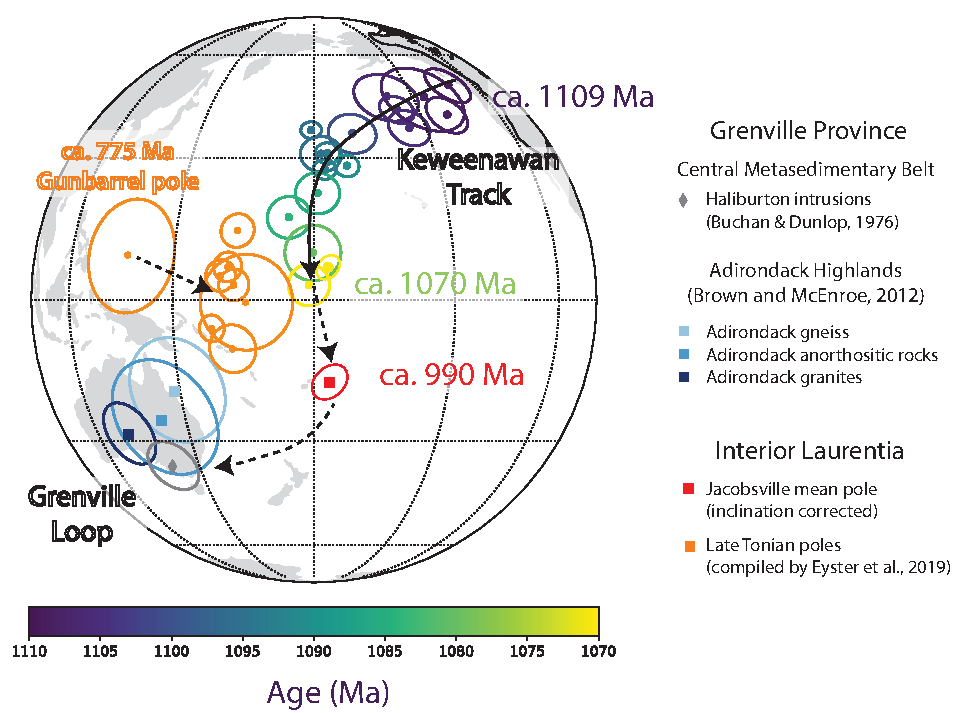
\includegraphics[width=\textwidth]{figure/Zhang2024a/Jacobsville_pole_plot.pdf}
\caption[Jacobsville Formation paleomagnetic pole position in context of the Keweenawan Track and the Grenville Loop]{The inclination-corrected Jacobsville Formation detrital remanent magnetization mean pole position with its Kent uncertainty ellipse is plotted in context of the ca. 1109-1070 Ma Keweenawan Track (poles color-coded by age shown in the colorbar), selected poles from the Grenville Province, and late Tonian poles of Laurentia as compiled by \cite{Eyster2019a} (orange colored poles). The southerly pole position of the ca. 990 Ma Jacobsville Formation indicates that the study area was crossing the equator in the late Mesoproterozoic to early Neoproterozoic. Given the large arc distance between the ca. 990 Ma Jacobsville pole and the poles of the Grenville loop, such as those of the the Haliburton intrusions, we suggest that estimates of their age as $>$1000 Ma \citep{Warnock2000a, Halls2015b, Evans2021b} are likely too old. The solid curve with arrow represents a continuous path of the Keweenawan Track, the dashed curves with arrow represent inferred apparent polar wander in the early Neoproterozoic based on data developed and compiled in this study and by \cite{Eyster2019a}. The pole compilation used in this figure is included as Table S1. }
\label{fig:pole_plot}
\end{figure*}

This slowdown in plate motion is geodynamically consistent with the onset of Grenvillian orogenesis. The earliest records of orogenesis on the leading margin of Laurentia occur ca. 1090 Ma with estimates of peak orogenesis associated with the Ottawan stage of the orogeny occurring ca. 1050 Ma \citep{Rivers2012a, Swanson-Hysell2023a}. Inversions of the Keweenawan Track that incorporate multiple tectonic Euler poles indicate a slowdown from rates exceeding 20 cm/yr prior to 1095 Ma to rates below 20 cm/yr after 1095 Ma \citep{Swanson-Hysell2019a, Rose2022a}. This initial slowdown could be associated with soft collision as contractional deformation initiated on the leading edge of Laurentia \citep{Staal2020a}. Continued contractional collision led to substantially thickened crust recorded by granulite-facies metamorphic rocks by the time of peak Ottawan phase metamorphism ca. 1050 Ma \citep{Rivers2012a}. The large slowdown in plate speed as now constrained by the Jacobsville paleomagnetic pole is associated with this progression to hard continent-continent collision involving increased crustal thickening and progressive transmission of contractional stress that eventually progressed into the interior of Laurentia \citep{Cannon1994a}.

Laurentia's rapid motion was associated with closure of the Unimos Ocean and is consistent with it being on the lower plate that subducted under a conjugate continent (e.g. Amazonia) that collided on its margin (\citealp{Swanson-Hysell2023a}; Fig. \ref{fig:Jacobsville_paleogeography}). The Jacobsville paleomagnetic pole constrains this motion to have slowed as orogeny progressed to be a large-scale continent-continent collision. As a result, Laurentia maintained a low-latitude position throughout the duration of the Grenvillian orogeny which sutured continents together into the supercontinent Rodinia (Fig. \ref{fig:Jacobsville_paleogeography}). 

\subsection{Implications for the age of the Grenville Loop}

Given that the age and pole position of the Jacobsville Formation had been uncertain and lacking other constraints from sedimentary or volcanic rocks, reconstruction of the paleogeography of Laurentia in the early Neoproterozoic has been reliant on paleomagnetic poles developed from metamorphic rocks within the Grenville Province \cite[e.g.][]{Weil1998a}. As is shown in Figure \ref{fig:pole_plot}, paleomagnetic poles of the Grenville Loop plot near Australia in present-day coordinates; forming arc distances ranging from $\sim$35\textdegree\ to more than 50\textdegree\ away from poles at the end of the ca. 1110 to 1070 Ma Keweenawan Track (Fig. \ref{fig:pole_plot}). Determining ages associated with the Grenville Loop poles is crucial for constraining the motion of Laurentia at this time and the configuration between Laurentia and hypothesized conjugate continents such as Baltica within Rodinia \citep{Cawood2017a, Gong2018a, Swanson-Hysell2021c}.

\begin{figure*}[h!]
\centering
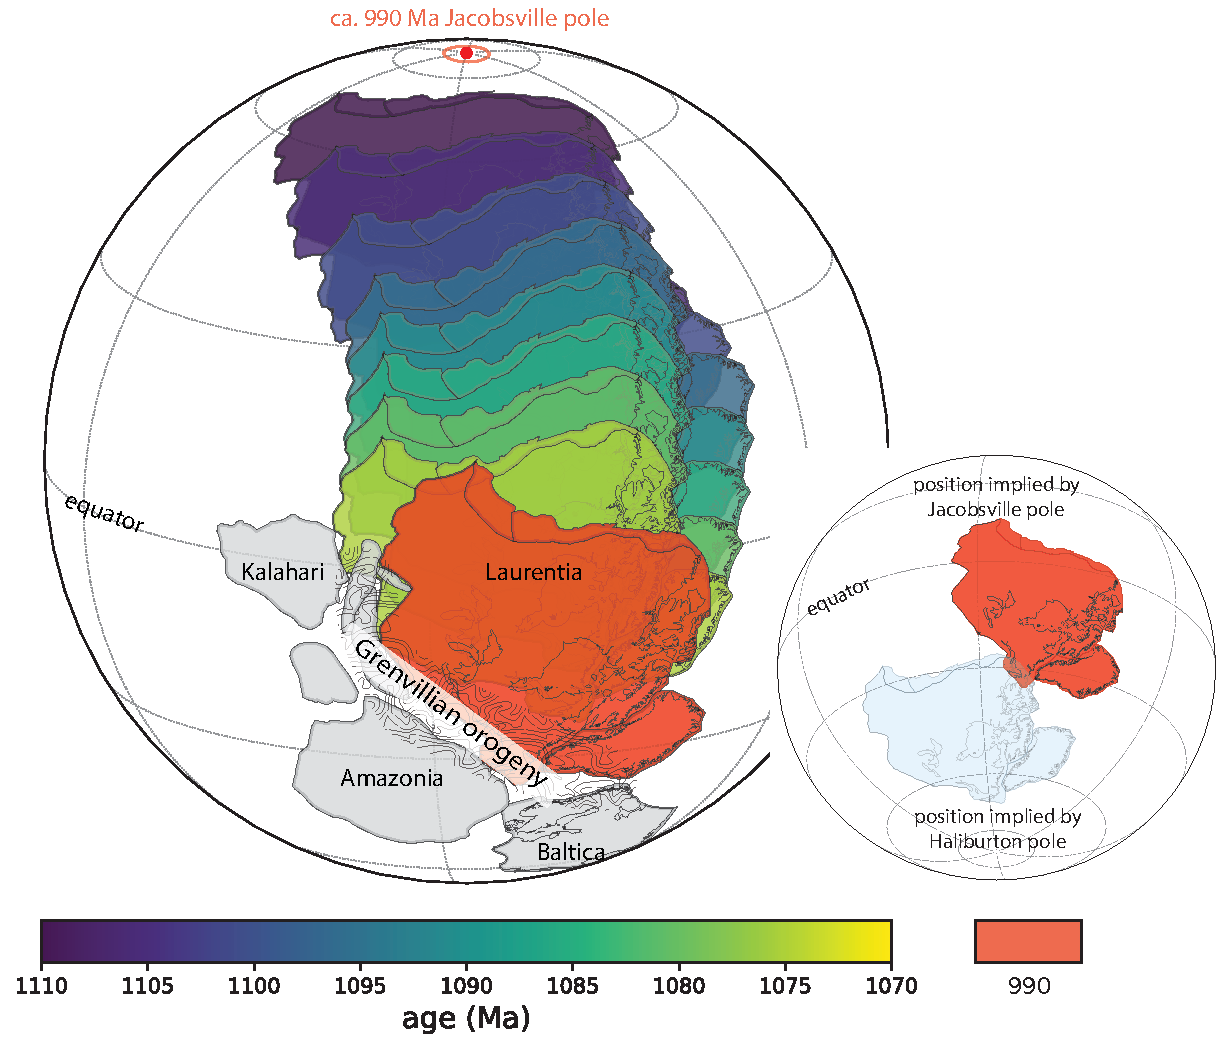
\includegraphics[width=0.8\textwidth]{figure/Zhang2024a/Jacobsville_paleogeography.pdf}
\caption[Paleogeographic position of Laurentia through the late Mesoproterozoic to early Neoproterozoic]{Paleogeographic position of Laurentia through the late Mesoproterozoic to early Neoproterozoic. The color-coded reconstructions show snapshots of Laurentia's position and orientation at 5 Myr intervals from 1110 to 1075 Ma. These reconstructions implement the two-stage tectonic Euler pole rotation inversion of \cite{Swanson-Hysell2019a}. The paleogeographic snapshot colored in red shows the position and orientation of Laurentia ca. 990 Ma as constrained by the Jacobsville paleomagnetic pole developed in this study. Interpreted positions of Laurentia's conjugate continents along its margin are shown in grey. This reconstruction shows that while Laurentia experienced rapid latitudinal changes through the Keweenawan Track that its motion was much slower between ca. 1075 and 990 Ma as the Grenvillian orogeny progressed. The paleogeographic positions of conjugate continents to Laurentia long the Grenville margin in the reconstructions follow the interpretation of \cite{Swanson-Hysell2023a}. The inset figure compares Laurentia's position predicted by the new Jacobsville paleomagnetic pole (red) and that constrained by the Haliburton intrusions of the Grenvillian orogeny (light blue) which has been assigned an age of 1015 Ma \citep{Warnock2000a}. We suggest that this and other Grenville loop poles are younger and that Laurentia traveled from low latitudes toward higher latitudes following ca. 990 Ma while the Grenville orogen was slowly cooling and exhuming.}
\label{fig:Jacobsville_paleogeography}
\end{figure*}

In contrast to rocks of the Midcontinent Rift where magnetizations can be confidently assigned to be the same age as the crystallization ages of the rocks \cite[e.g.][]{Davis1997a,Fairchild2017a,Swanson-Hysell2019a}, rocks of the Grenville orogen experienced up to granulite facies metamorphism (temperatures $>$900\textdegree C; \citealp[e.g.][]{Shinevar2021a, Metzger2021a}) and acquired magnetic remanence during subsequent exhumation \citep{McWilliams1975a, Dunlop1985a, Dodson1985a}. During slow post-orogenic exhumation (1-3\textdegree C/Myr; \citealp[e.g.][]{Rivers2023a}), magnetic minerals acquired remanence by cooling through an extended temperature range over millions to tens of millions of years \citep{Pullaiah1975a, Dodson1980a} or by crystallizing through exsolution \citep{McEnroe2007a}. Determining the age of magnetization in such rocks requires reconstructing cooling histories using isotopic thermochronometers which experience radioisotopic accumulation on mineral-specific closure of elemental diffusion \citep{Dodson1973a, Dodson1985a}. 

Based on the interpretation that blocking of magnetic remanence of the magnetite-bearing Haliburton intrusions of the Grenville Central Metamorphic Belt occurred during relatively narrow temperature ranges close to the Curie temperature of magnetite (i.e. 580\textdegree C), \cite{Warnock2000a} considered that the timing of remanence acquisition during cooling of the intrusions is bracketed between U-Pb titanite and $^{40}$Ar/$^{39}$Ar hornblende dates. As a result, that study interpreted the age associated with the Haliburton paleomagnetic pole to be ca. 1015 Ma. This age has been assigned to the pole in subsequent compilations \cite[e.g.][]{Evans2021a}. In the central Adirondack Highlands of the Grenville orogen, magnetite-bearing granitic rocks and anorthositic rocks record pole positions that overlap with the Haliburton pole while their ages have been interpreted by \cite{Brown2012a} to be ca. 990-970 Ma, based on U-Pb and $^{40}$Ar/$^{39}$Ar thermochronology data developed by \cite{Mezger1991a}. The ca. 990 Ma Jacobsville pole position is both distinct from the Grenville Loop poles and is consistent with a slowdown of Laurentia's plate motion associated with the Grenvillian orogeny (Fig. \ref{fig:pole_plot}). If ages that have been assigned to Grenville Loop poles are taken at face value, those poles represent the position of Laurentia both before and after the position constrained by the ca. 990 Ma Jacobsville pole. Such an interpretation would imply either rapid plate tectonic motion of Laurentia coeval with the Rigolet phase of the Grenvillian orogeny or rapid oscillatory true polar wander \cite[e.g.][]{Evans2003a}. A more straightforward alternative model that could explain the distinct pole positions between the Jacobsville pole and the Grenville Loop poles is that the poles from the Grenville orogen are younger than currently interpreted. Instead of having acquired remanence during the orogeny, the Grenville rocks could have acquired magnetic remanence during protracted exhumation that followed the ca. 980 Ma cessation of contractional deformation associated with the Rigolet stage of the orogeny. In this scenario, the migration of Rodinia to the higher latitude position represented by the Grenville loop poles would have occurred further into the Neoproterozoic after the Grenvillian orogeny had ceased.  

While numerous paleomagnetic data sets have been developed from rocks of the Grenville Province, few are paired with well-calibrated, high-precision thermochronology data. Recent data sets, such as new apatite U-Pb dates of 923 $\pm$ 14 Ma (2$\sigma$ analytical uncertainty) from the Wilberforce pyroxenite \citep{Paul2021a}, give tantalizing hints that temperatures that blocked magnetizations in portions of the orogen were achieved later than the ages assigned to paleomagnetic poles would suggest as U-Pb apatite closure temperatures are close to magnetite blocking temperatures (ca. 360-570\textdegree C; \citealp{Cherniak1991a}). To test the hypothesis that the Grenville Loop is younger than in previous interpretations, geochronology studies are needed to exploit the resolving power of high-precision whole grain analytical methods (i.e. ID-TIMS) and high-spatial-resolution in-situ methods (e.g. laser ablation depth profiling; \citealp{Chew2021a}) for reconstructing the cooling rate and time-temperature history of the Grenville Province. Testing this hypothesis is critical for reconstructions of the paleogeography of Rodinia in the early Neoproterozoic. 

\section{Conclusion}

The magnetization of hematite-bearing fine-grained siliciclastic sedimentary rocks from the Jacobsville Formation can be shown to be detrital and primary through positive intraformational conglomerate and fold tests. We use these data to develop a new inclination-corrected paleomagnetic pole that can be constrained with recently published radiometric age constraints from \cite{Hodgin2022a} to be ca. 990 Ma. This high-quality pole is a crucial addition to Laurentia's apparent polar wander path in the earliest Neoproterozoic. Its position indicates that Laurentia's plate motion significantly slowed during Grenvillian collisional orogenesis. The new pole establishes a well-calibrated constraint for the position of the supercontinent Rodinia in early Neoproterozoic with Laurentia being at the center. The Jacobsville pole implies that ages associated with the paleomagnetic poles recorded by metamorphic rocks of the Grenville Province are likely younger than in current interpretations. Further paired studies of high-quality paleomagnetism and high-precision thermochronology are needed to illuminate Rodinia's motion and configuration in the early Neoproterozoic. 


\section{Acknowledgments}
Project research was funded by NSF CAREER grant EAR-1847277. Jim DeGraff provided helpful guidance in identifying exposures of the Jacobsville Formation. We gratefully acknowledge the Michigan Department of Natural Resources for sampling permitting. We thank Tim Lyons for additional private land access. We thank Madeline Swanson-Hysell for her assistance in the field. We thank David Malone, Douglas Elmore, and two anonymous reviewers for their helpful reviews. 
